\documentclass[11pt]{article}
\usepackage[textwidth=18.0cm, textheight=23.0cm, top=2.0cm]{geometry}
\usepackage{pst-all}
\usepackage{amssymb}
\usepackage{tikz}
\usepackage{underscore}\begin{document}
\pagestyle{empty}


ClassName: \underline{\textbf{Class_03.2bp-46}}
\par
BinSize: \underline{\textbf{40 × 40}}
\par
ReduceSize: \underline{\textbf{40 × 40}}
\par
TypeNum: \underline{\textbf{97}}
\par
Num: \underline{\textbf{100}}
\par
OutS: \underline{\textbf{32000}}
\par
InS: \underline{\textbf{29445}}
\par
Rate: \underline{\textbf{0.920}}
\par
UB: \underline{\textbf{20}}
\par
LB0: \underline{\textbf{20}}
\par
LB: \underline{\textbf{20}}
\par
LBWithCut: \underline{\textbf{20}}
\par
NodeCut: \underline{\textbf{0}}
\par
ExtendedNodeCnt: \underline{\textbf{1}}
\par
GenNodeCnt: \underline{\textbf{1}}
\par
PrimalNode: \underline{\textbf{0}}
\par
ColumnCount: \underline{\textbf{20}}
\par
TotalCutCount: \underline{\textbf{0}}
\par
RootCutCount: \underline{\textbf{0}}
\par
LPSolverCnt: \underline{\textbf{1}}
\par
PricingSolverCnt: \underline{\textbf{0}}
\par
BranchAndBoundNum: \underline{\textbf{1}}
\par
isOpt: \underline{\textbf{true}}
\par
TimeOnInitSolution: \underline{\textbf{0.190 s}}
\par
TimeOnPrimal: \underline{\textbf{0.000 s}}
\par
TimeOnPricing: \underline{\textbf{0.000 s}}
\par
TimeOnRmp: \underline{\textbf{0.078 s}}
\par
TotalTime: \underline{\textbf{0.331 s}}
\par
\newpage


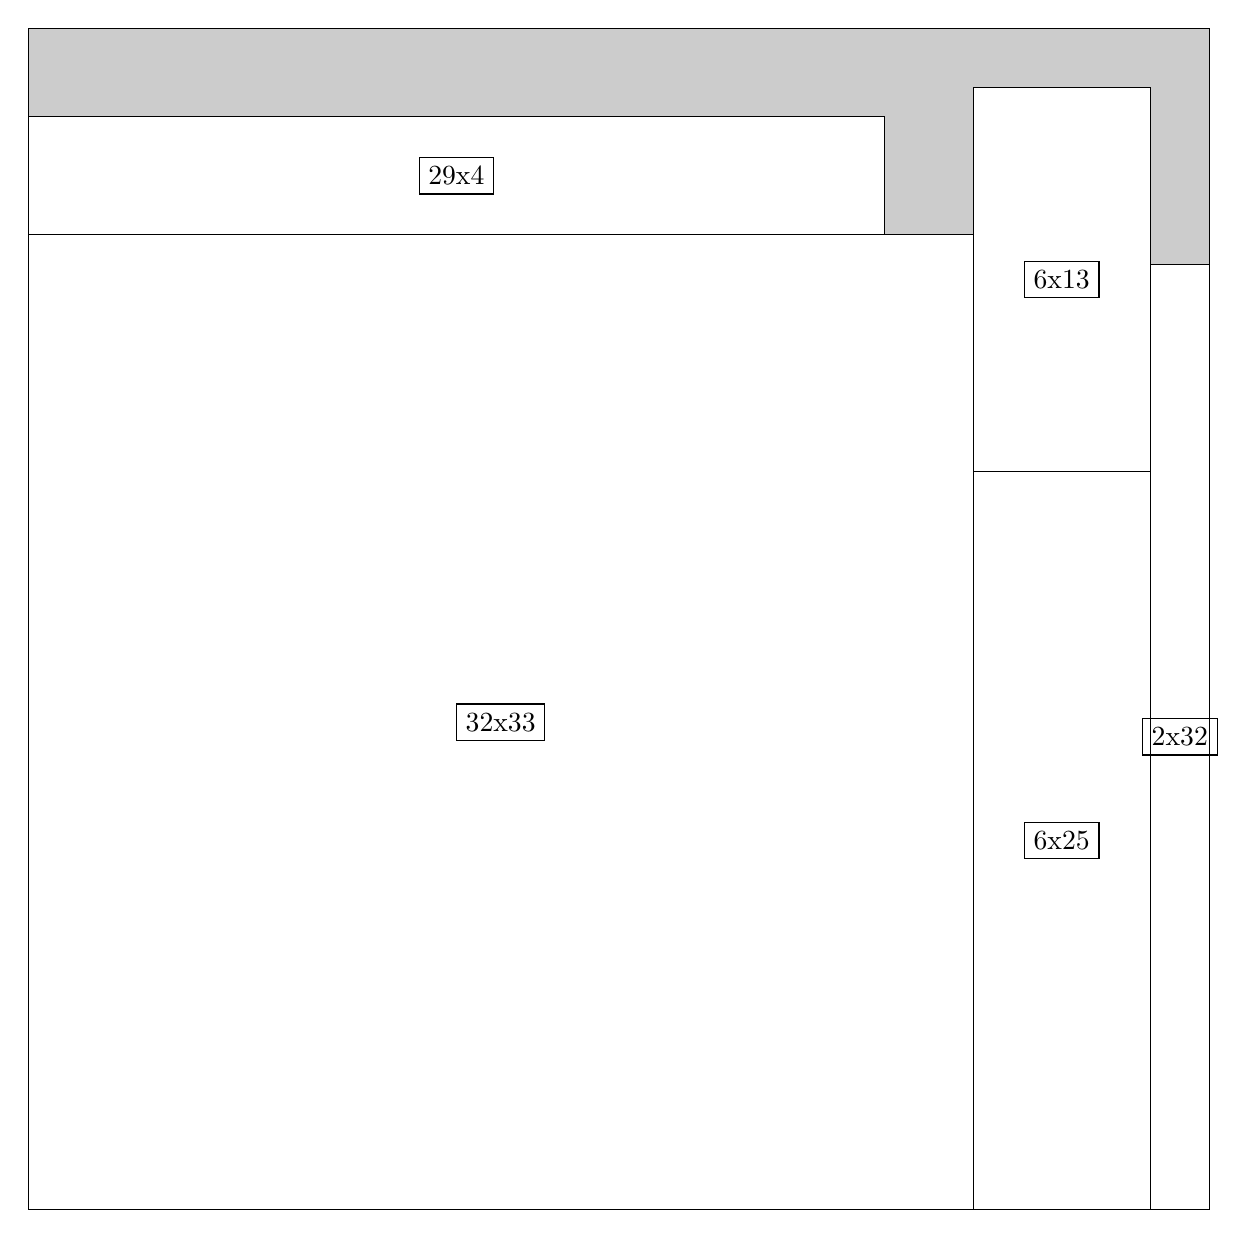
\begin{tikzpicture}[shorten >=1pt,scale=1.0,every node/.style={scale=1.0},->]
\tikzstyle{vertex}=[circle,fill=black!25,minimum size=14pt,inner sep=0pt]
\filldraw[fill=gray!40!white, draw=black] (0,0) rectangle (15.0,15.0);
\foreach \name/\x/\y/\w/\h in {32x33/0.0/0.0/12.0/12.375,6x25/12.0/0.0/2.25/9.375,29x4/0.0/12.375/10.875/1.5,6x13/12.0/9.375/2.25/4.875,2x32/14.25/0.0/0.75/12.0}
\filldraw[fill=white!40!white, draw=black] (\x,\y) rectangle node[draw] (\name) {\name} ++(\w,\h);
\end{tikzpicture}


w =32 , h =33 , x =0 , y =0 , v =1056
\par
w =6 , h =25 , x =32 , y =0 , v =150
\par
w =29 , h =4 , x =0 , y =33 , v =116
\par
w =6 , h =13 , x =32 , y =25 , v =78
\par
w =2 , h =32 , x =38 , y =0 , v =64
\par
\newpage


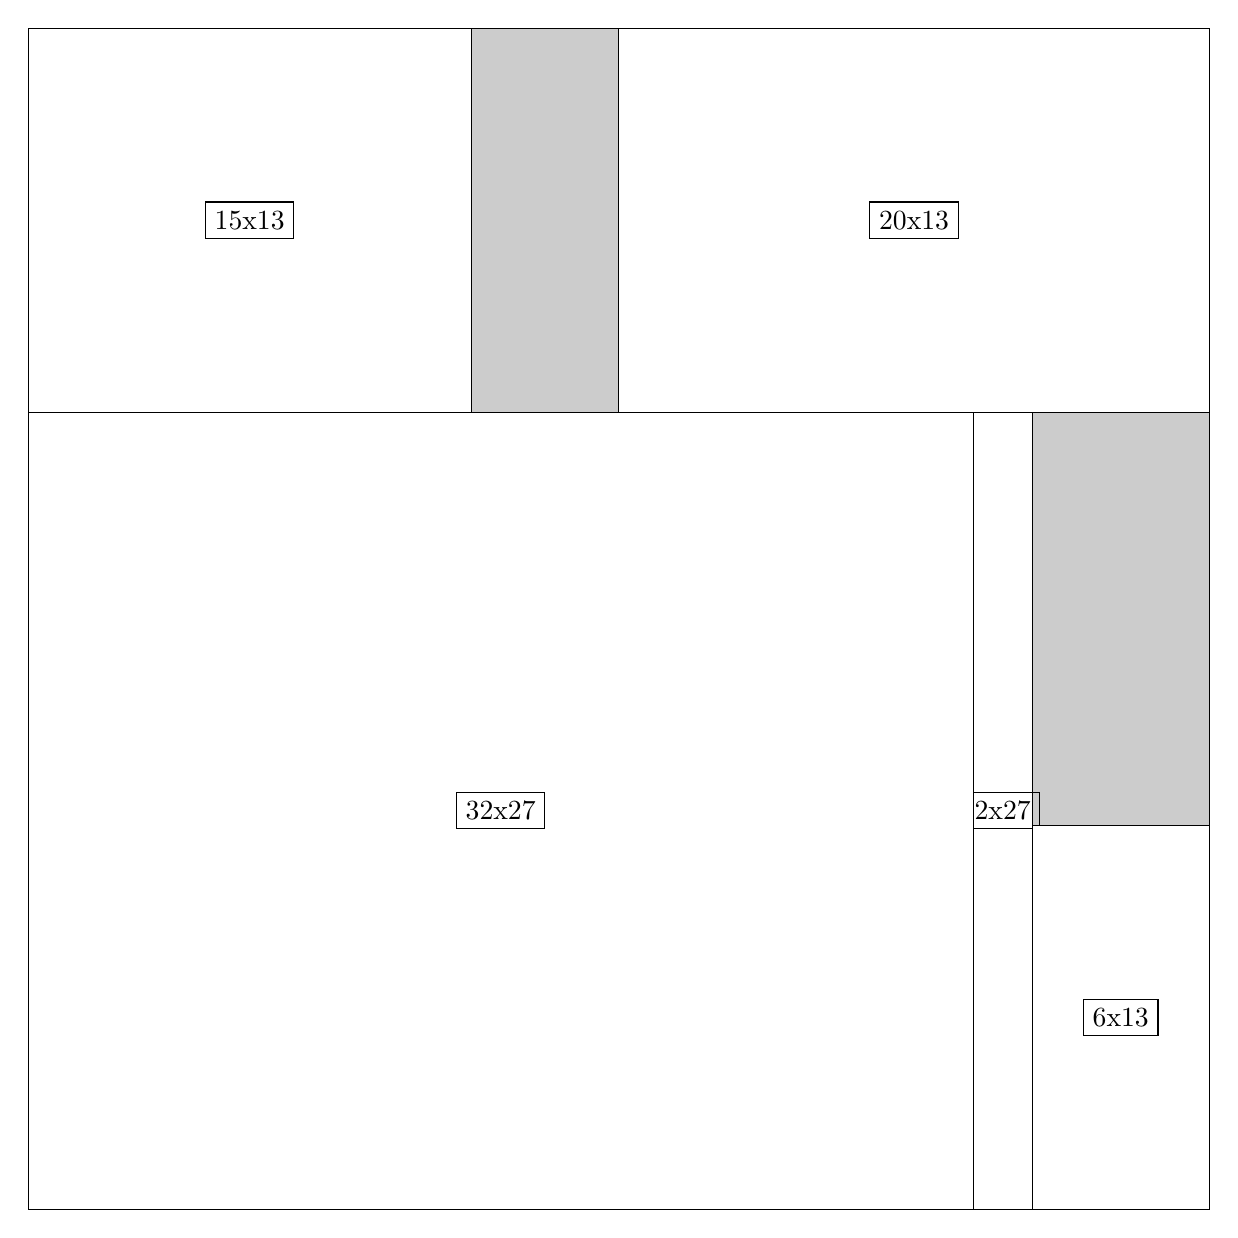
\begin{tikzpicture}[shorten >=1pt,scale=1.0,every node/.style={scale=1.0},->]
\tikzstyle{vertex}=[circle,fill=black!25,minimum size=14pt,inner sep=0pt]
\filldraw[fill=gray!40!white, draw=black] (0,0) rectangle (15.0,15.0);
\foreach \name/\x/\y/\w/\h in {2x27/12.0/0.0/0.75/10.125,32x27/0.0/0.0/12.0/10.125,20x13/7.5/10.125/7.5/4.875,15x13/0.0/10.125/5.625/4.875,6x13/12.75/0.0/2.25/4.875}
\filldraw[fill=white!40!white, draw=black] (\x,\y) rectangle node[draw] (\name) {\name} ++(\w,\h);
\end{tikzpicture}


w =2 , h =27 , x =32 , y =0 , v =54
\par
w =32 , h =27 , x =0 , y =0 , v =864
\par
w =20 , h =13 , x =20 , y =27 , v =260
\par
w =15 , h =13 , x =0 , y =27 , v =195
\par
w =6 , h =13 , x =34 , y =0 , v =78
\par
\newpage


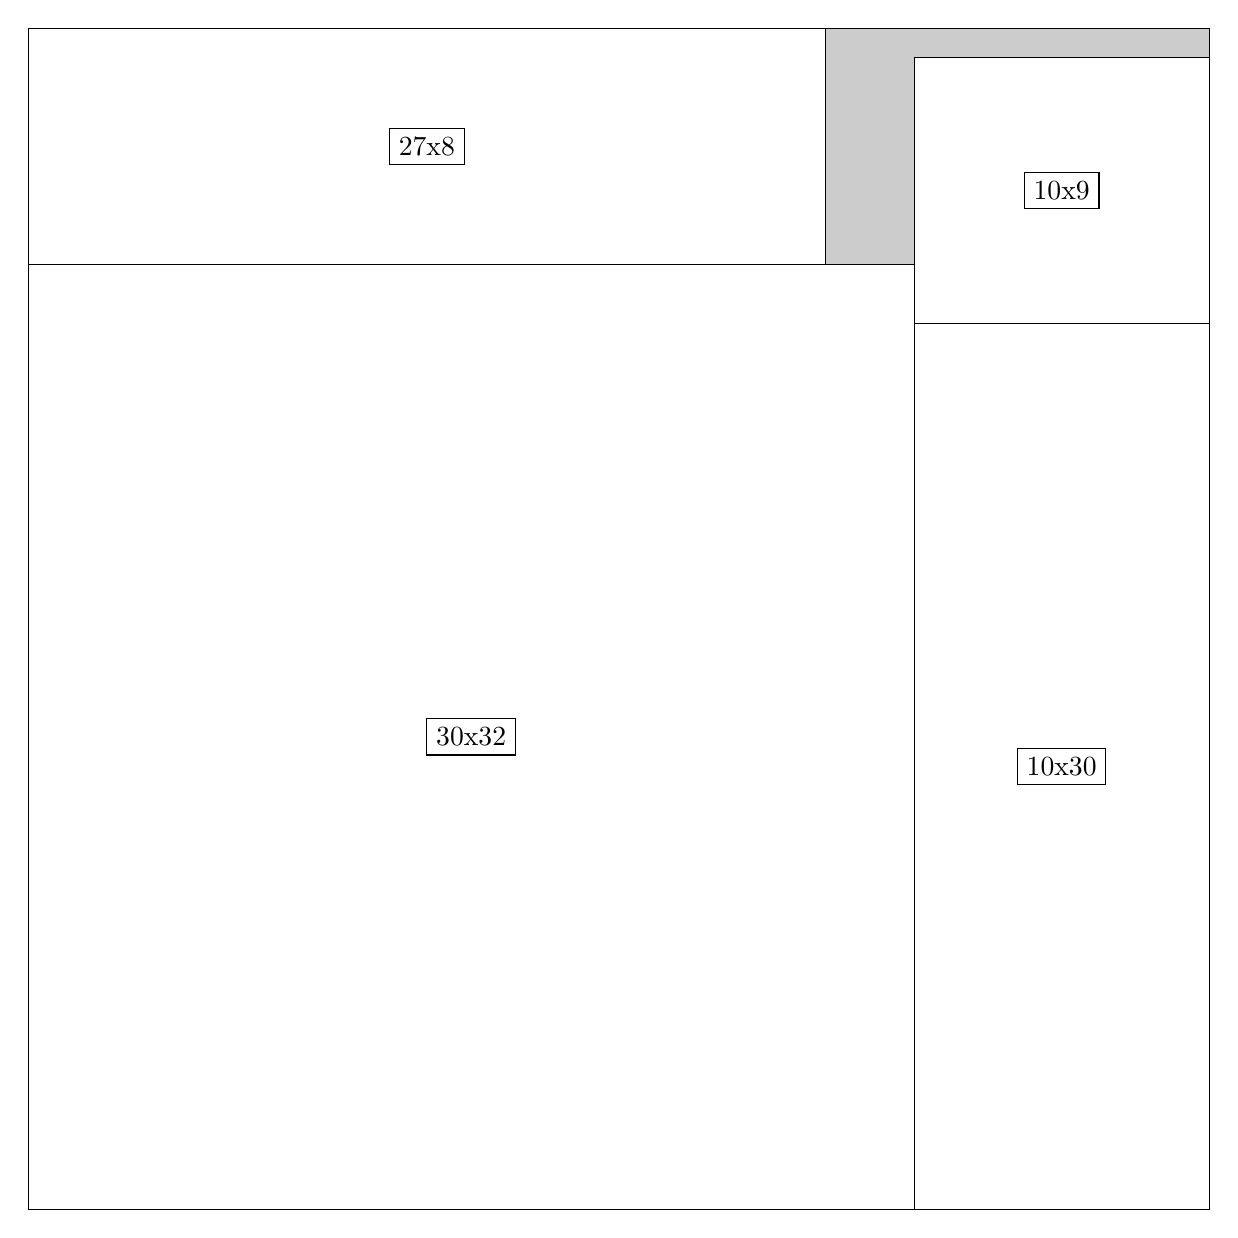
\begin{tikzpicture}[shorten >=1pt,scale=1.0,every node/.style={scale=1.0},->]
\tikzstyle{vertex}=[circle,fill=black!25,minimum size=14pt,inner sep=0pt]
\filldraw[fill=gray!40!white, draw=black] (0,0) rectangle (15.0,15.0);
\foreach \name/\x/\y/\w/\h in {30x32/0.0/0.0/11.25/12.0,10x30/11.25/0.0/3.75/11.25,27x8/0.0/12.0/10.125/3.0,10x9/11.25/11.25/3.75/3.375}
\filldraw[fill=white!40!white, draw=black] (\x,\y) rectangle node[draw] (\name) {\name} ++(\w,\h);
\end{tikzpicture}


w =30 , h =32 , x =0 , y =0 , v =960
\par
w =10 , h =30 , x =30 , y =0 , v =300
\par
w =27 , h =8 , x =0 , y =32 , v =216
\par
w =10 , h =9 , x =30 , y =30 , v =90
\par
\newpage


\begin{tikzpicture}[shorten >=1pt,scale=1.0,every node/.style={scale=1.0},->]
\tikzstyle{vertex}=[circle,fill=black!25,minimum size=14pt,inner sep=0pt]
\filldraw[fill=gray!40!white, draw=black] (0,0) rectangle (15.0,15.0);
\foreach \name/\x/\y/\w/\h in {28x34/0.0/0.0/10.5/12.75,12x32/10.5/0.0/4.5/12.0,28x6/0.0/12.75/10.5/2.25,7x8/10.5/12.0/2.625/3.0,2x8/13.125/12.0/0.75/3.0,3x5/13.875/12.0/1.125/1.875}
\filldraw[fill=white!40!white, draw=black] (\x,\y) rectangle node[draw] (\name) {\name} ++(\w,\h);
\end{tikzpicture}


w =28 , h =34 , x =0 , y =0 , v =952
\par
w =12 , h =32 , x =28 , y =0 , v =384
\par
w =28 , h =6 , x =0 , y =34 , v =168
\par
w =7 , h =8 , x =28 , y =32 , v =56
\par
w =2 , h =8 , x =35 , y =32 , v =16
\par
w =3 , h =5 , x =37 , y =32 , v =15
\par
\newpage


\begin{tikzpicture}[shorten >=1pt,scale=1.0,every node/.style={scale=1.0},->]
\tikzstyle{vertex}=[circle,fill=black!25,minimum size=14pt,inner sep=0pt]
\filldraw[fill=gray!40!white, draw=black] (0,0) rectangle (15.0,15.0);
\foreach \name/\x/\y/\w/\h in {28x33/0.0/0.0/10.5/12.375,11x26/10.875/5.25/4.125/9.75,12x14/10.5/0.0/4.5/5.25,15x7/4.875/12.375/5.625/2.625,7x7/2.25/12.375/2.625/2.625,1x22/10.5/5.25/0.375/8.25,3x7/1.125/12.375/1.125/2.625,2x3/0.0/12.375/0.75/1.125,1x4/10.5/13.5/0.375/1.5,2x1/0.0/13.5/0.75/0.375}
\filldraw[fill=white!40!white, draw=black] (\x,\y) rectangle node[draw] (\name) {\name} ++(\w,\h);
\end{tikzpicture}


w =28 , h =33 , x =0 , y =0 , v =924
\par
w =11 , h =26 , x =29 , y =14 , v =286
\par
w =12 , h =14 , x =28 , y =0 , v =168
\par
w =15 , h =7 , x =13 , y =33 , v =105
\par
w =7 , h =7 , x =6 , y =33 , v =49
\par
w =1 , h =22 , x =28 , y =14 , v =22
\par
w =3 , h =7 , x =3 , y =33 , v =21
\par
w =2 , h =3 , x =0 , y =33 , v =6
\par
w =1 , h =4 , x =28 , y =36 , v =4
\par
w =2 , h =1 , x =0 , y =36 , v =2
\par
\newpage


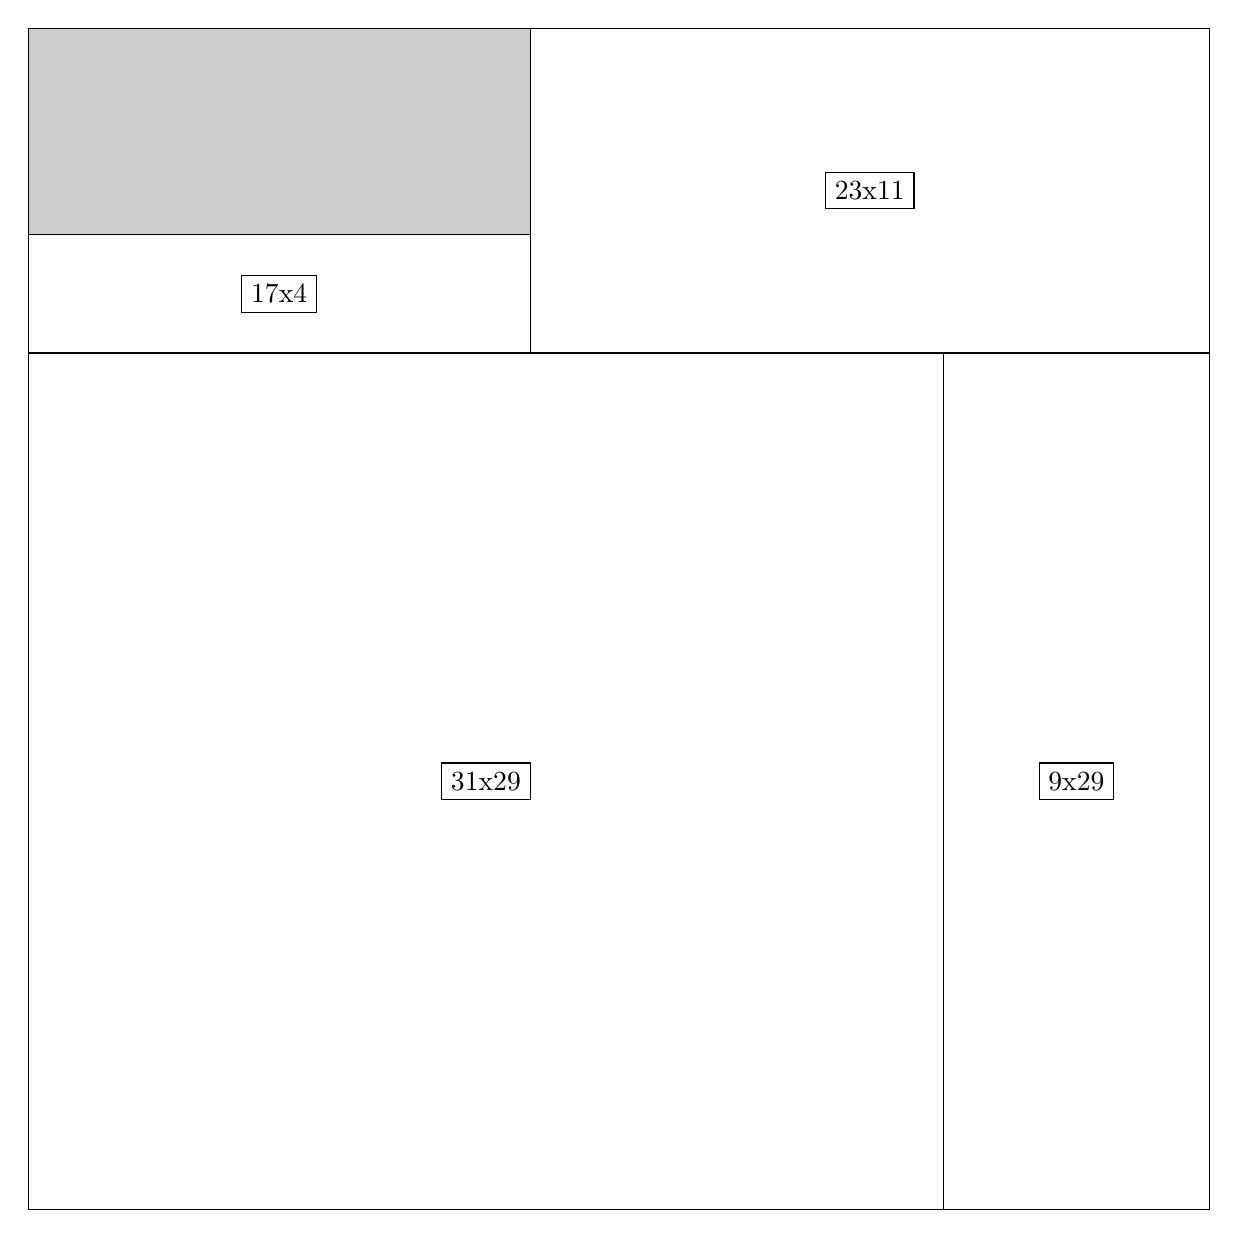
\begin{tikzpicture}[shorten >=1pt,scale=1.0,every node/.style={scale=1.0},->]
\tikzstyle{vertex}=[circle,fill=black!25,minimum size=14pt,inner sep=0pt]
\filldraw[fill=gray!40!white, draw=black] (0,0) rectangle (15.0,15.0);
\foreach \name/\x/\y/\w/\h in {31x29/0.0/0.0/11.625/10.875,9x29/11.625/0.0/3.375/10.875,23x11/6.375/10.875/8.625/4.125,17x4/0.0/10.875/6.375/1.5}
\filldraw[fill=white!40!white, draw=black] (\x,\y) rectangle node[draw] (\name) {\name} ++(\w,\h);
\end{tikzpicture}


w =31 , h =29 , x =0 , y =0 , v =899
\par
w =9 , h =29 , x =31 , y =0 , v =261
\par
w =23 , h =11 , x =17 , y =29 , v =253
\par
w =17 , h =4 , x =0 , y =29 , v =68
\par
\newpage


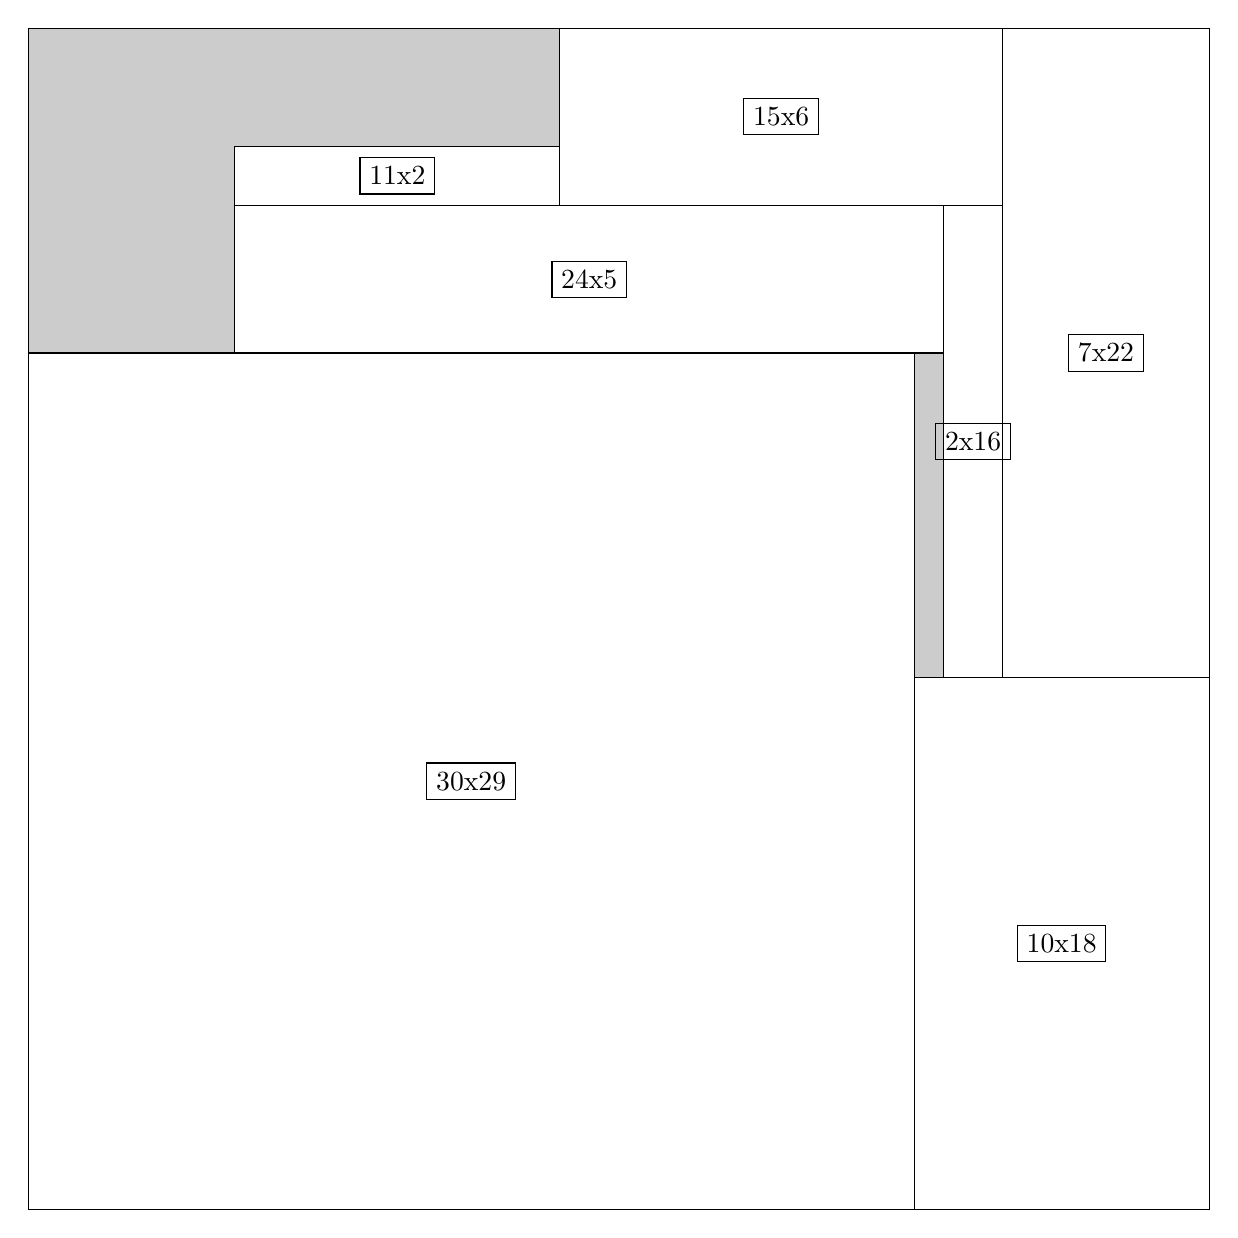
\begin{tikzpicture}[shorten >=1pt,scale=1.0,every node/.style={scale=1.0},->]
\tikzstyle{vertex}=[circle,fill=black!25,minimum size=14pt,inner sep=0pt]
\filldraw[fill=gray!40!white, draw=black] (0,0) rectangle (15.0,15.0);
\foreach \name/\x/\y/\w/\h in {30x29/0.0/0.0/11.25/10.875,10x18/11.25/0.0/3.75/6.75,7x22/12.375/6.75/2.625/8.25,24x5/2.625/10.875/9.0/1.875,15x6/6.75/12.75/5.625/2.25,2x16/11.625/6.75/0.75/6.0,11x2/2.625/12.75/4.125/0.75}
\filldraw[fill=white!40!white, draw=black] (\x,\y) rectangle node[draw] (\name) {\name} ++(\w,\h);
\end{tikzpicture}


w =30 , h =29 , x =0 , y =0 , v =870
\par
w =10 , h =18 , x =30 , y =0 , v =180
\par
w =7 , h =22 , x =33 , y =18 , v =154
\par
w =24 , h =5 , x =7 , y =29 , v =120
\par
w =15 , h =6 , x =18 , y =34 , v =90
\par
w =2 , h =16 , x =31 , y =18 , v =32
\par
w =11 , h =2 , x =7 , y =34 , v =22
\par
\newpage


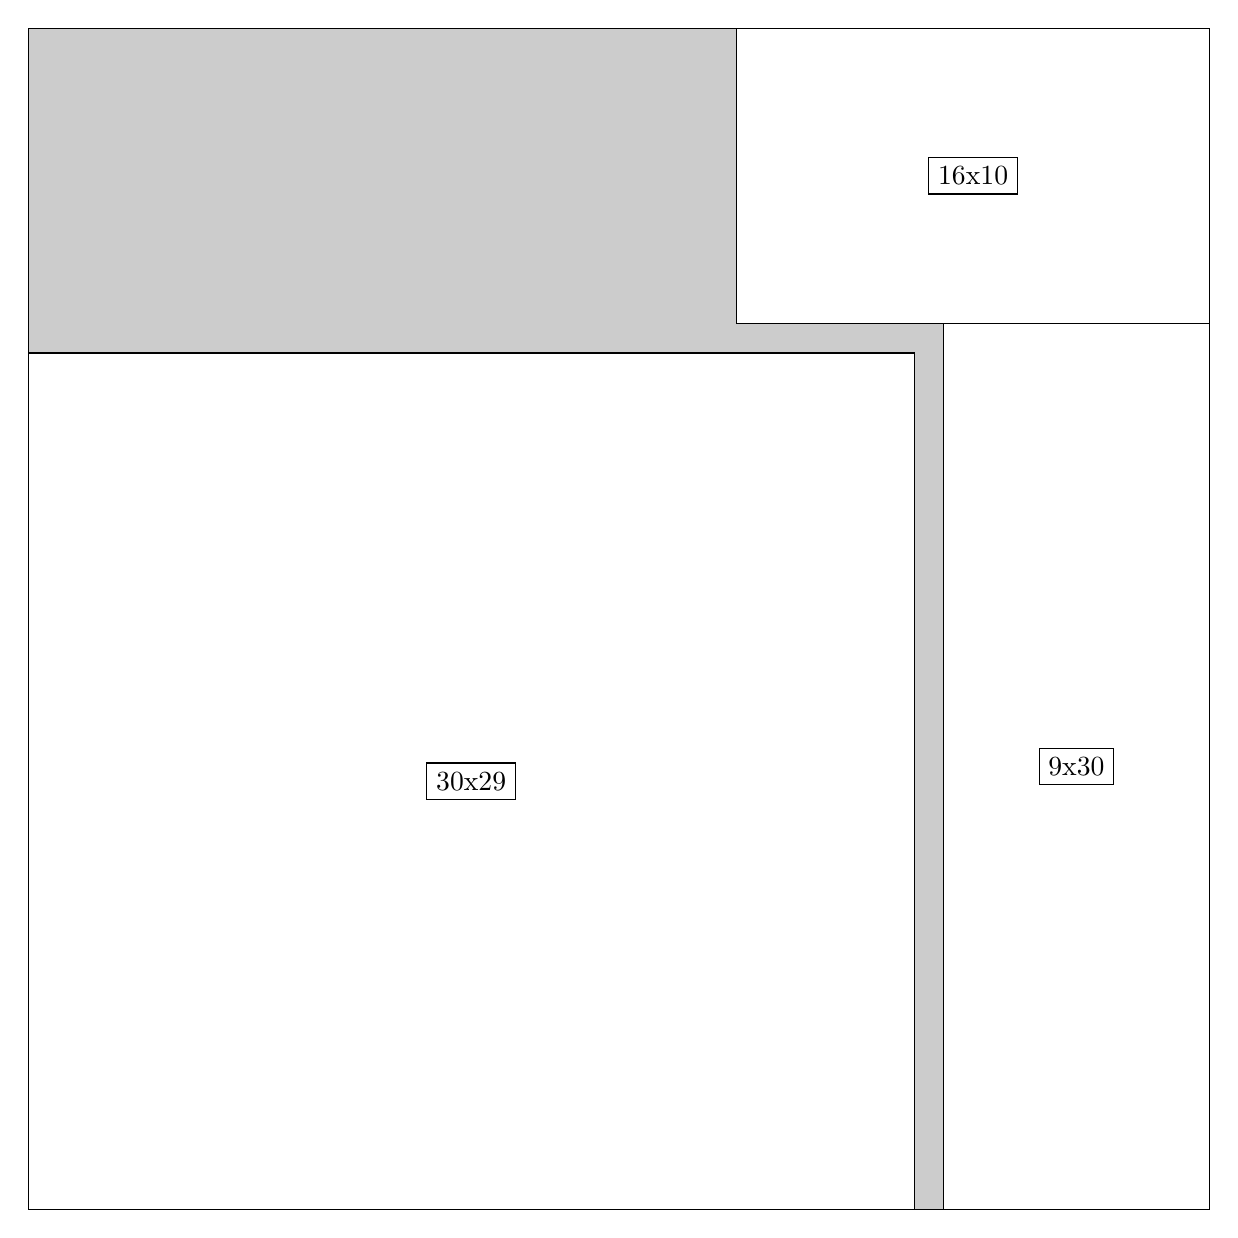
\begin{tikzpicture}[shorten >=1pt,scale=1.0,every node/.style={scale=1.0},->]
\tikzstyle{vertex}=[circle,fill=black!25,minimum size=14pt,inner sep=0pt]
\filldraw[fill=gray!40!white, draw=black] (0,0) rectangle (15.0,15.0);
\foreach \name/\x/\y/\w/\h in {30x29/0.0/0.0/11.25/10.875,9x30/11.625/0.0/3.375/11.25,16x10/9.0/11.25/6.0/3.75}
\filldraw[fill=white!40!white, draw=black] (\x,\y) rectangle node[draw] (\name) {\name} ++(\w,\h);
\end{tikzpicture}


w =30 , h =29 , x =0 , y =0 , v =870
\par
w =9 , h =30 , x =31 , y =0 , v =270
\par
w =16 , h =10 , x =24 , y =30 , v =160
\par
\newpage


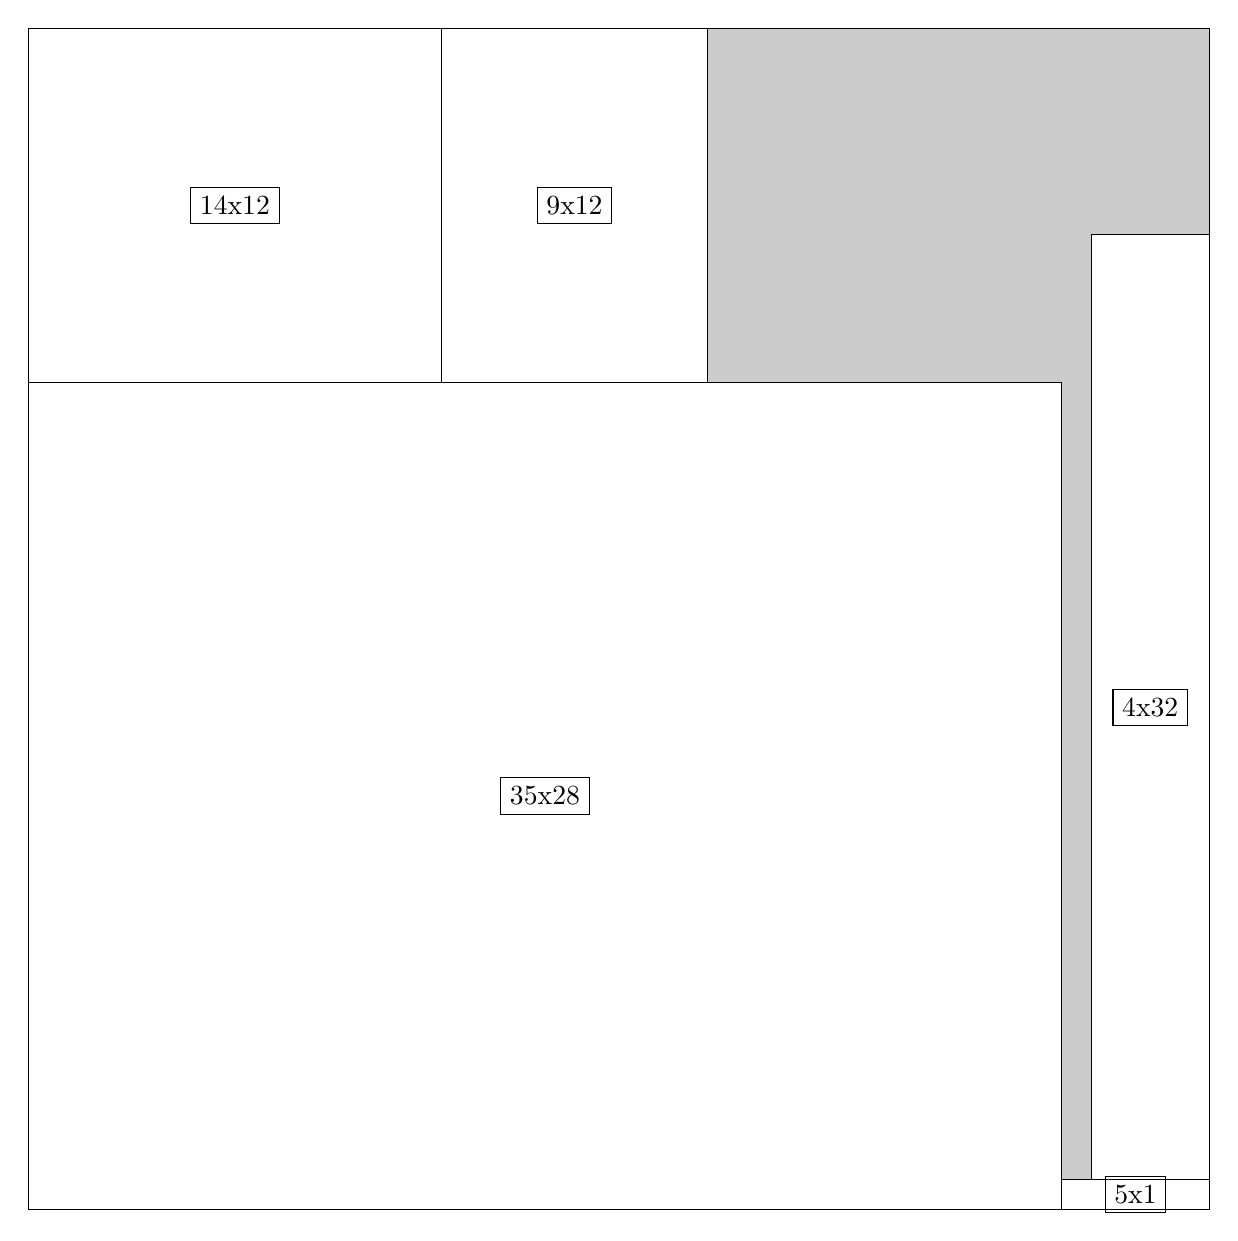
\begin{tikzpicture}[shorten >=1pt,scale=1.0,every node/.style={scale=1.0},->]
\tikzstyle{vertex}=[circle,fill=black!25,minimum size=14pt,inner sep=0pt]
\filldraw[fill=gray!40!white, draw=black] (0,0) rectangle (15.0,15.0);
\foreach \name/\x/\y/\w/\h in {14x12/0.0/10.5/5.25/4.5,4x32/13.5/0.375/1.5/12.0,9x12/5.25/10.5/3.375/4.5,35x28/0.0/0.0/13.125/10.5,5x1/13.125/0.0/1.875/0.375}
\filldraw[fill=white!40!white, draw=black] (\x,\y) rectangle node[draw] (\name) {\name} ++(\w,\h);
\end{tikzpicture}


w =14 , h =12 , x =0 , y =28 , v =168
\par
w =4 , h =32 , x =36 , y =1 , v =128
\par
w =9 , h =12 , x =14 , y =28 , v =108
\par
w =35 , h =28 , x =0 , y =0 , v =980
\par
w =5 , h =1 , x =35 , y =0 , v =5
\par
\newpage


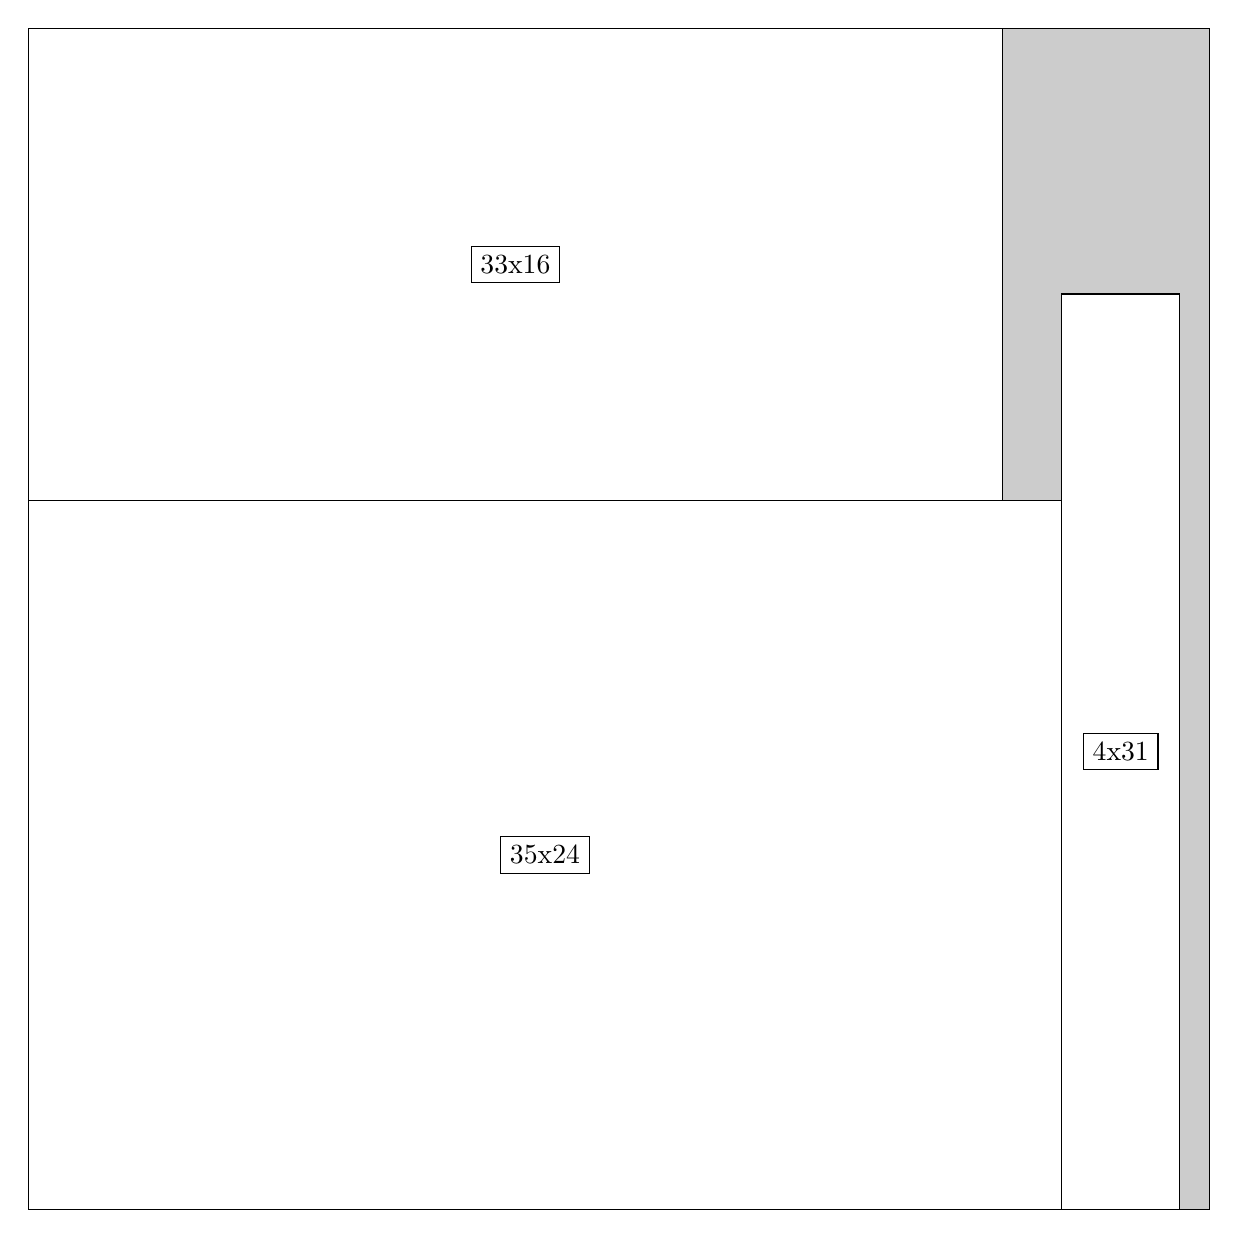
\begin{tikzpicture}[shorten >=1pt,scale=1.0,every node/.style={scale=1.0},->]
\tikzstyle{vertex}=[circle,fill=black!25,minimum size=14pt,inner sep=0pt]
\filldraw[fill=gray!40!white, draw=black] (0,0) rectangle (15.0,15.0);
\foreach \name/\x/\y/\w/\h in {35x24/0.0/0.0/13.125/9.0,33x16/0.0/9.0/12.375/6.0,4x31/13.125/0.0/1.5/11.625}
\filldraw[fill=white!40!white, draw=black] (\x,\y) rectangle node[draw] (\name) {\name} ++(\w,\h);
\end{tikzpicture}


w =35 , h =24 , x =0 , y =0 , v =840
\par
w =33 , h =16 , x =0 , y =24 , v =528
\par
w =4 , h =31 , x =35 , y =0 , v =124
\par
\newpage


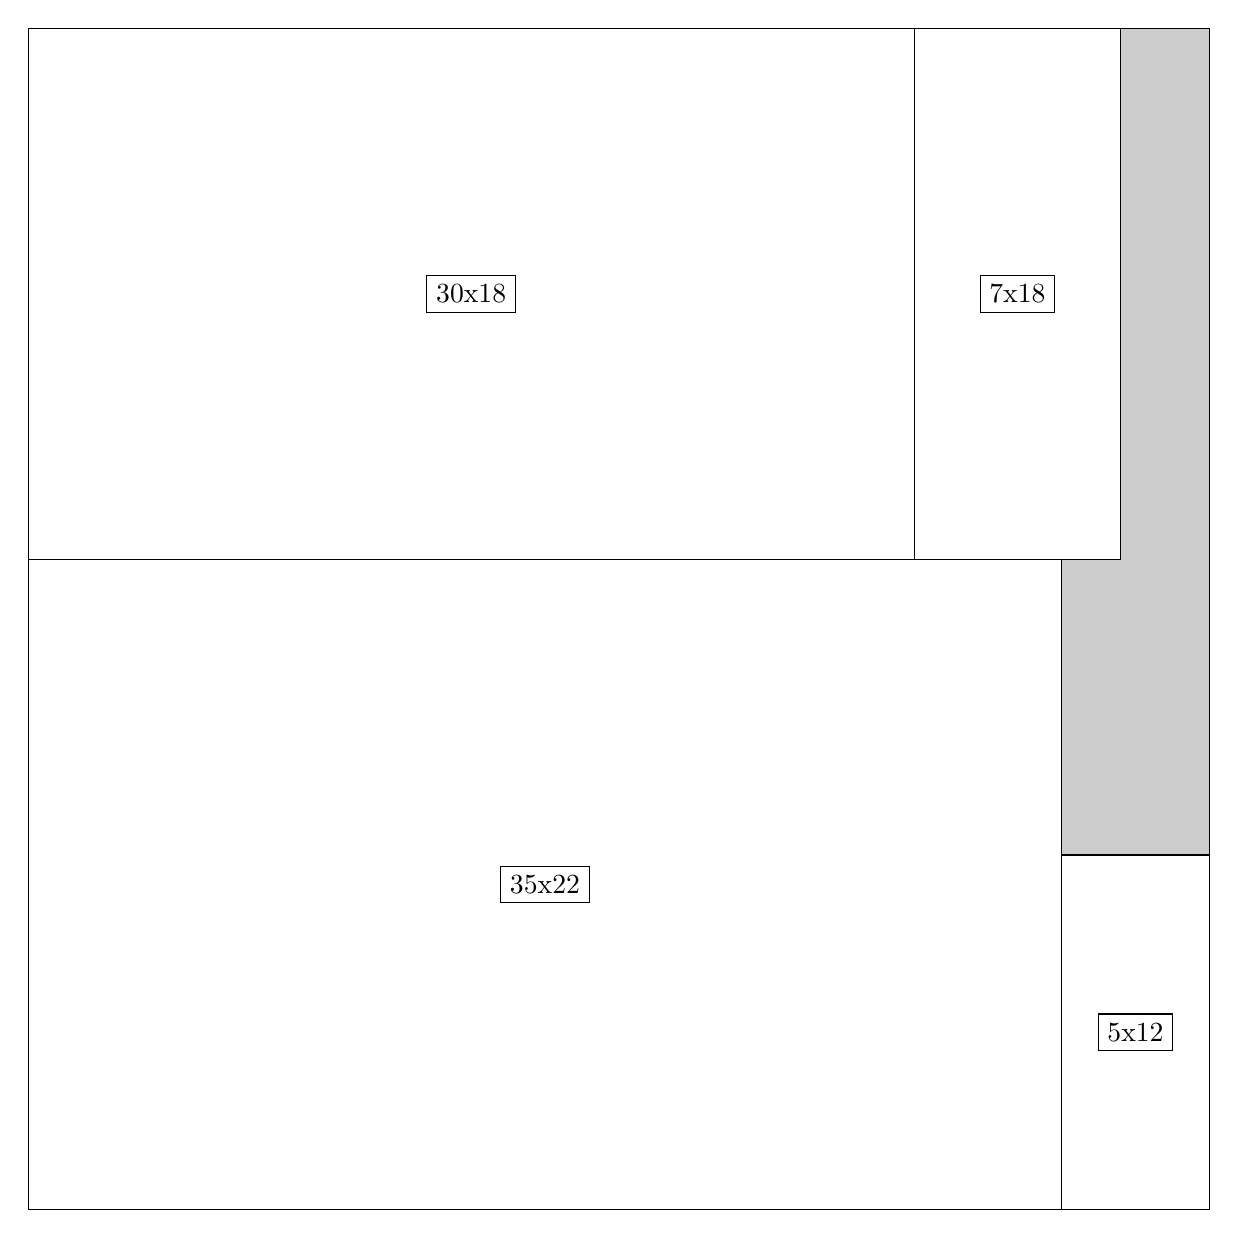
\begin{tikzpicture}[shorten >=1pt,scale=1.0,every node/.style={scale=1.0},->]
\tikzstyle{vertex}=[circle,fill=black!25,minimum size=14pt,inner sep=0pt]
\filldraw[fill=gray!40!white, draw=black] (0,0) rectangle (15.0,15.0);
\foreach \name/\x/\y/\w/\h in {35x22/0.0/0.0/13.125/8.25,30x18/0.0/8.25/11.25/6.75,7x18/11.25/8.25/2.625/6.75,5x12/13.125/0.0/1.875/4.5}
\filldraw[fill=white!40!white, draw=black] (\x,\y) rectangle node[draw] (\name) {\name} ++(\w,\h);
\end{tikzpicture}


w =35 , h =22 , x =0 , y =0 , v =770
\par
w =30 , h =18 , x =0 , y =22 , v =540
\par
w =7 , h =18 , x =30 , y =22 , v =126
\par
w =5 , h =12 , x =35 , y =0 , v =60
\par
\newpage


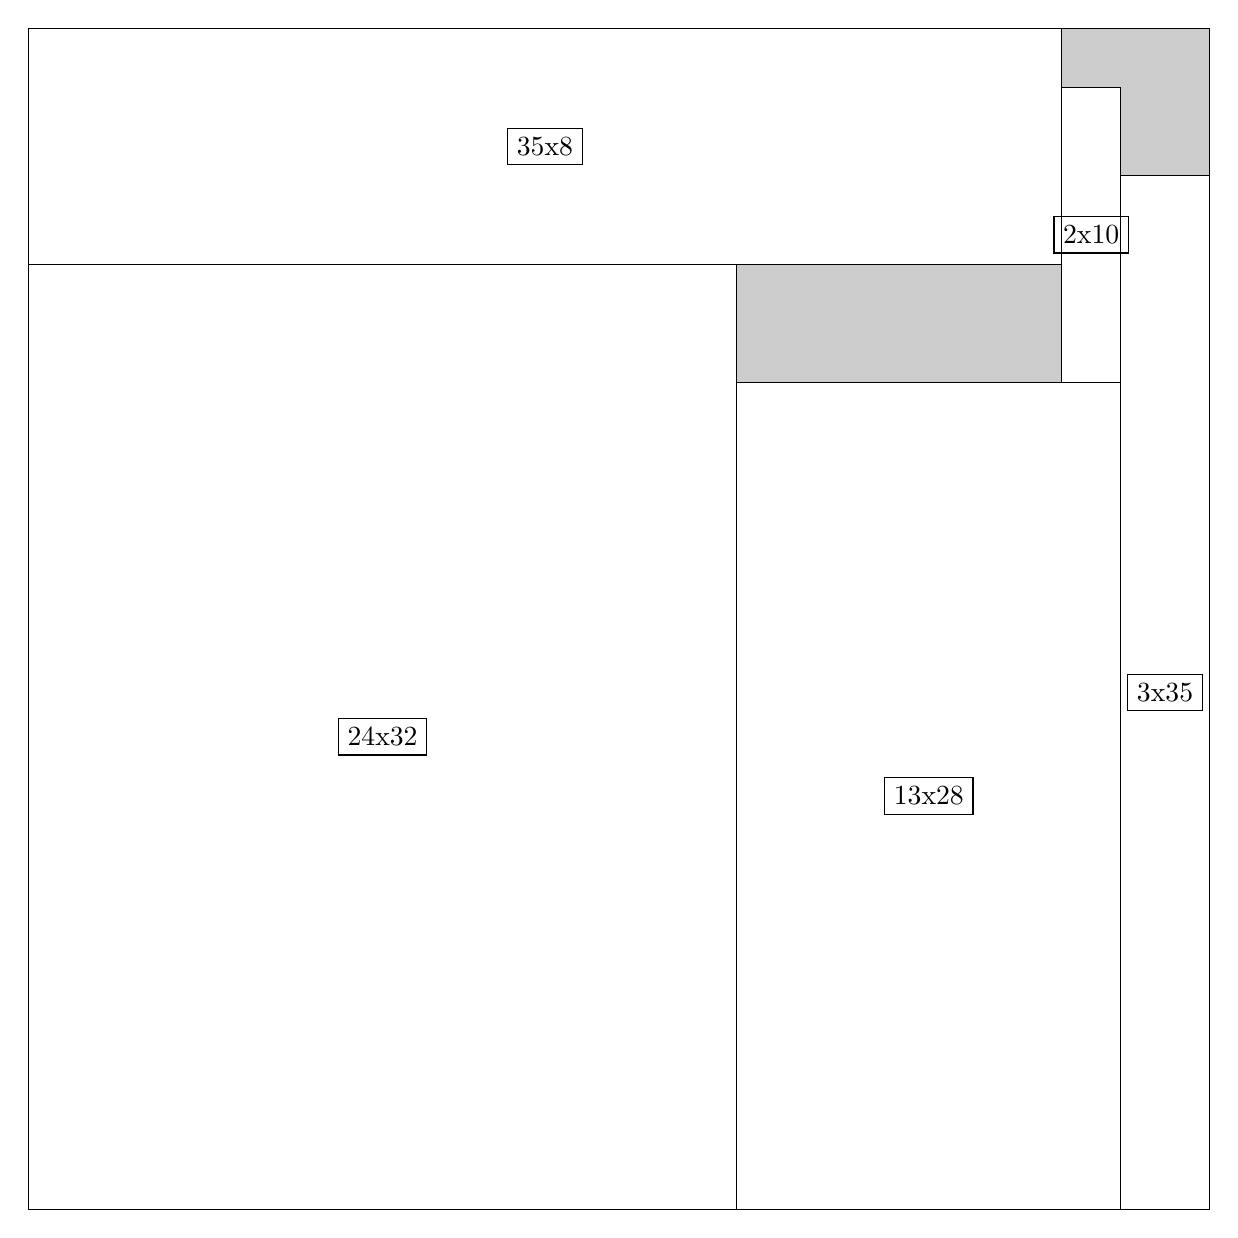
\begin{tikzpicture}[shorten >=1pt,scale=1.0,every node/.style={scale=1.0},->]
\tikzstyle{vertex}=[circle,fill=black!25,minimum size=14pt,inner sep=0pt]
\filldraw[fill=gray!40!white, draw=black] (0,0) rectangle (15.0,15.0);
\foreach \name/\x/\y/\w/\h in {24x32/0.0/0.0/9.0/12.0,13x28/9.0/0.0/4.875/10.5,35x8/0.0/12.0/13.125/3.0,3x35/13.875/0.0/1.125/13.125,2x10/13.125/10.5/0.75/3.75}
\filldraw[fill=white!40!white, draw=black] (\x,\y) rectangle node[draw] (\name) {\name} ++(\w,\h);
\end{tikzpicture}


w =24 , h =32 , x =0 , y =0 , v =768
\par
w =13 , h =28 , x =24 , y =0 , v =364
\par
w =35 , h =8 , x =0 , y =32 , v =280
\par
w =3 , h =35 , x =37 , y =0 , v =105
\par
w =2 , h =10 , x =35 , y =28 , v =20
\par
\newpage


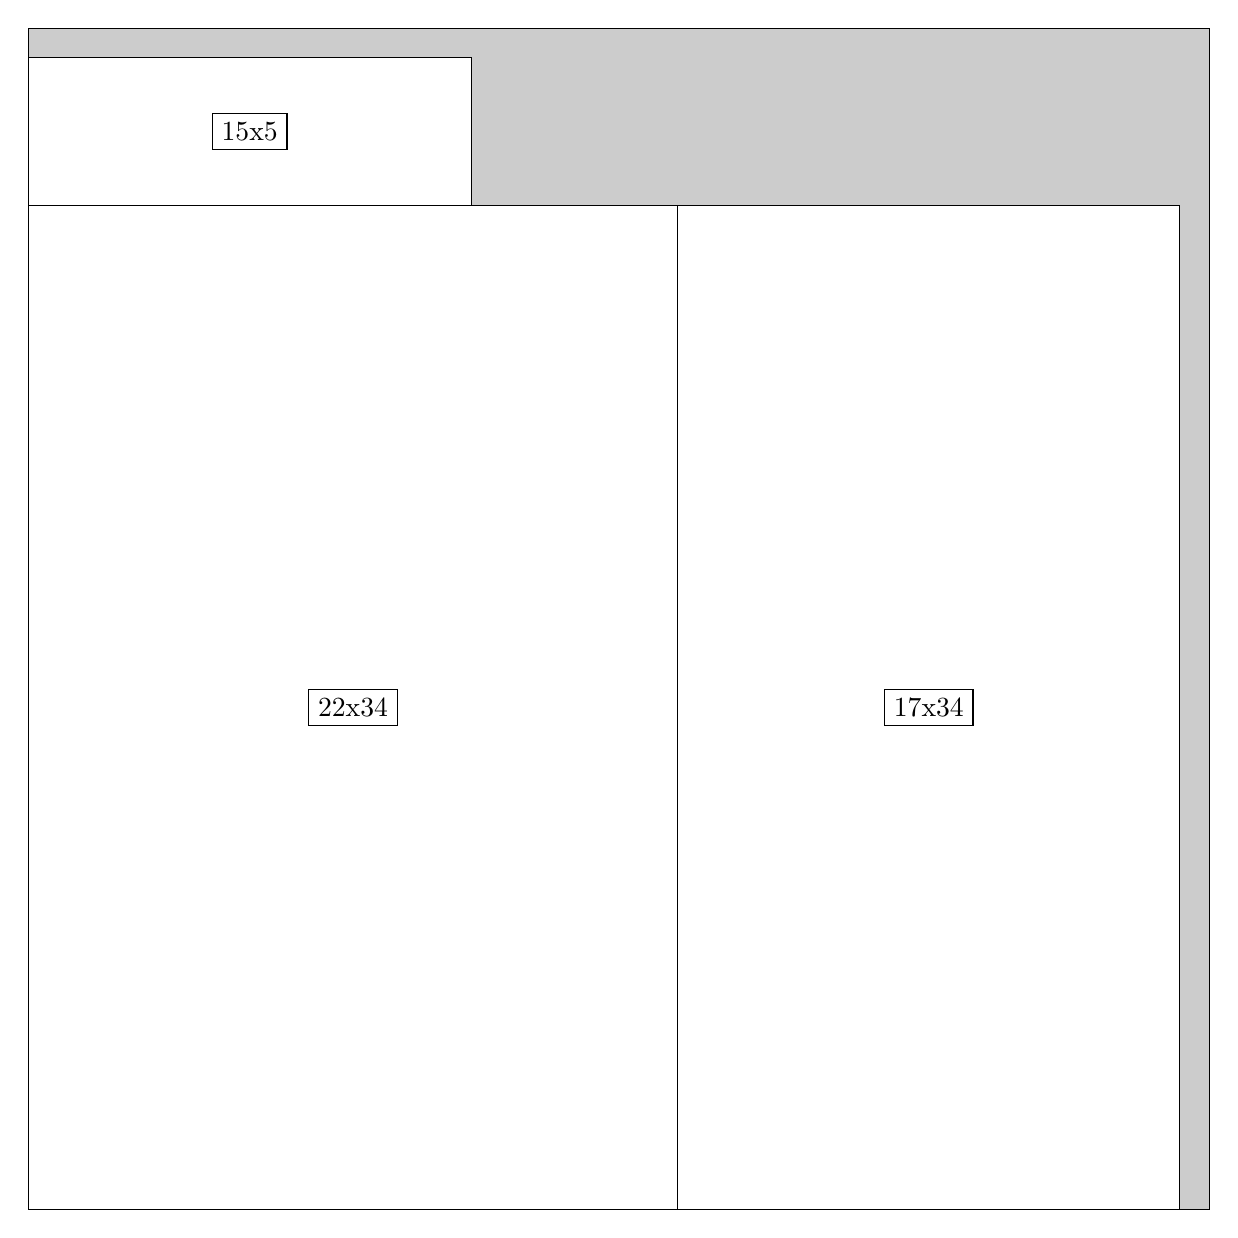
\begin{tikzpicture}[shorten >=1pt,scale=1.0,every node/.style={scale=1.0},->]
\tikzstyle{vertex}=[circle,fill=black!25,minimum size=14pt,inner sep=0pt]
\filldraw[fill=gray!40!white, draw=black] (0,0) rectangle (15.0,15.0);
\foreach \name/\x/\y/\w/\h in {22x34/0.0/0.0/8.25/12.75,17x34/8.25/0.0/6.375/12.75,15x5/0.0/12.75/5.625/1.875}
\filldraw[fill=white!40!white, draw=black] (\x,\y) rectangle node[draw] (\name) {\name} ++(\w,\h);
\end{tikzpicture}


w =22 , h =34 , x =0 , y =0 , v =748
\par
w =17 , h =34 , x =22 , y =0 , v =578
\par
w =15 , h =5 , x =0 , y =34 , v =75
\par
\newpage


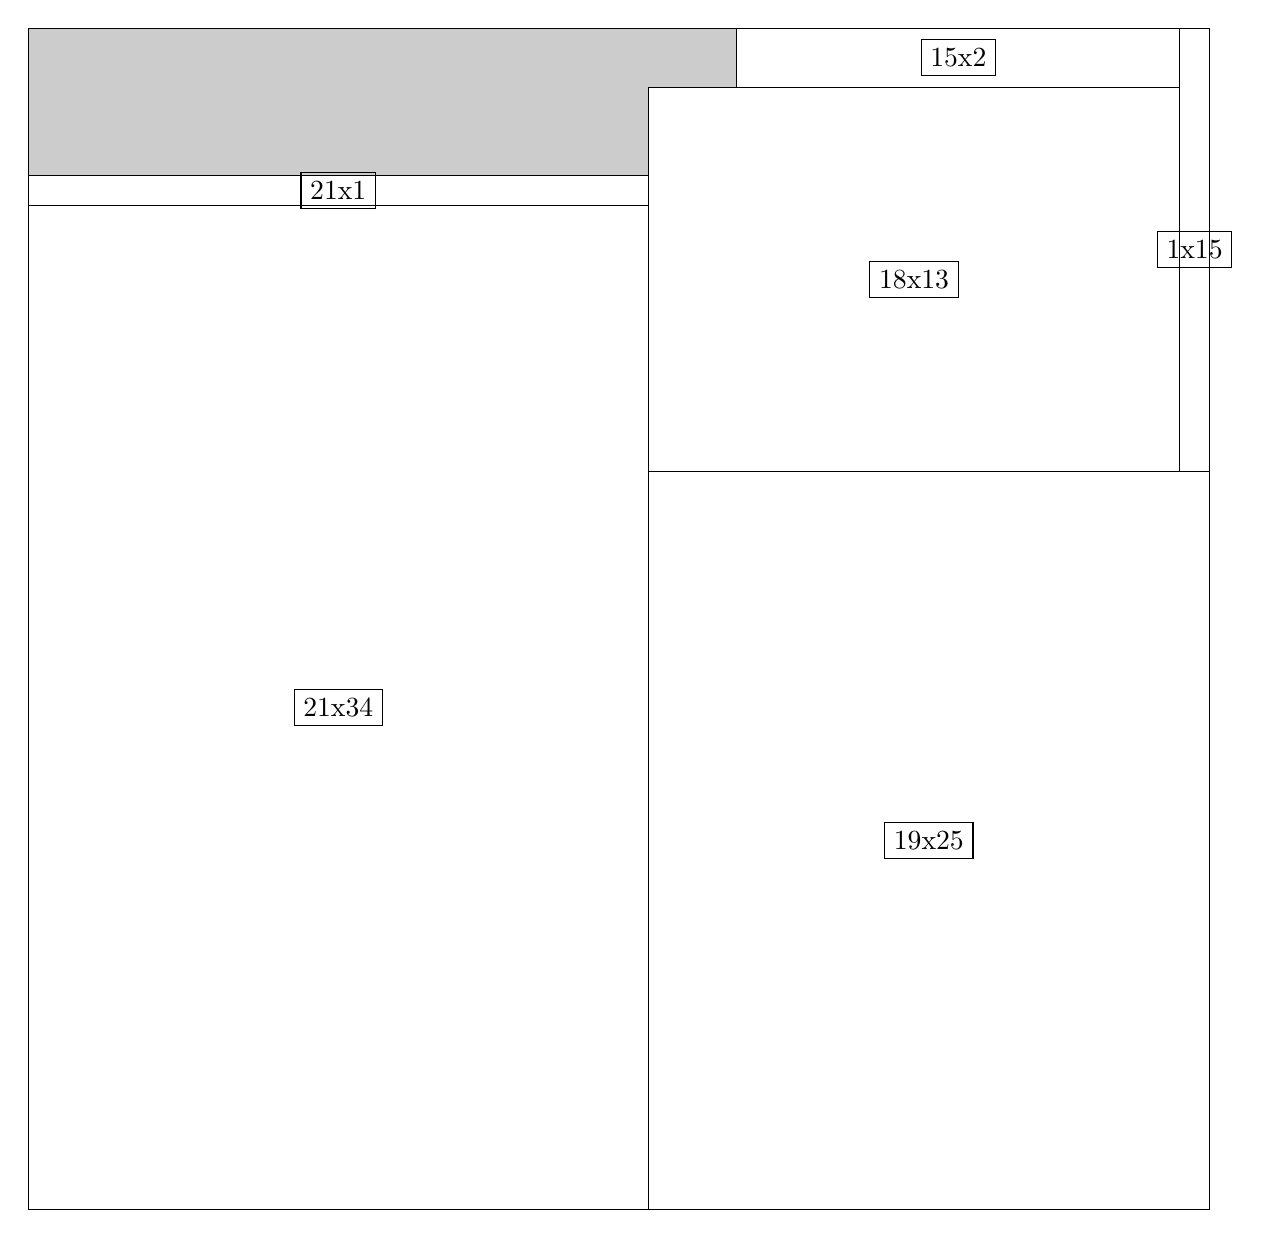
\begin{tikzpicture}[shorten >=1pt,scale=1.0,every node/.style={scale=1.0},->]
\tikzstyle{vertex}=[circle,fill=black!25,minimum size=14pt,inner sep=0pt]
\filldraw[fill=gray!40!white, draw=black] (0,0) rectangle (15.0,15.0);
\foreach \name/\x/\y/\w/\h in {21x34/0.0/0.0/7.875/12.75,19x25/7.875/0.0/7.125/9.375,18x13/7.875/9.375/6.75/4.875,15x2/9.0/14.25/5.625/0.75,21x1/0.0/12.75/7.875/0.375,1x15/14.625/9.375/0.375/5.625}
\filldraw[fill=white!40!white, draw=black] (\x,\y) rectangle node[draw] (\name) {\name} ++(\w,\h);
\end{tikzpicture}


w =21 , h =34 , x =0 , y =0 , v =714
\par
w =19 , h =25 , x =21 , y =0 , v =475
\par
w =18 , h =13 , x =21 , y =25 , v =234
\par
w =15 , h =2 , x =24 , y =38 , v =30
\par
w =21 , h =1 , x =0 , y =34 , v =21
\par
w =1 , h =15 , x =39 , y =25 , v =15
\par
\newpage


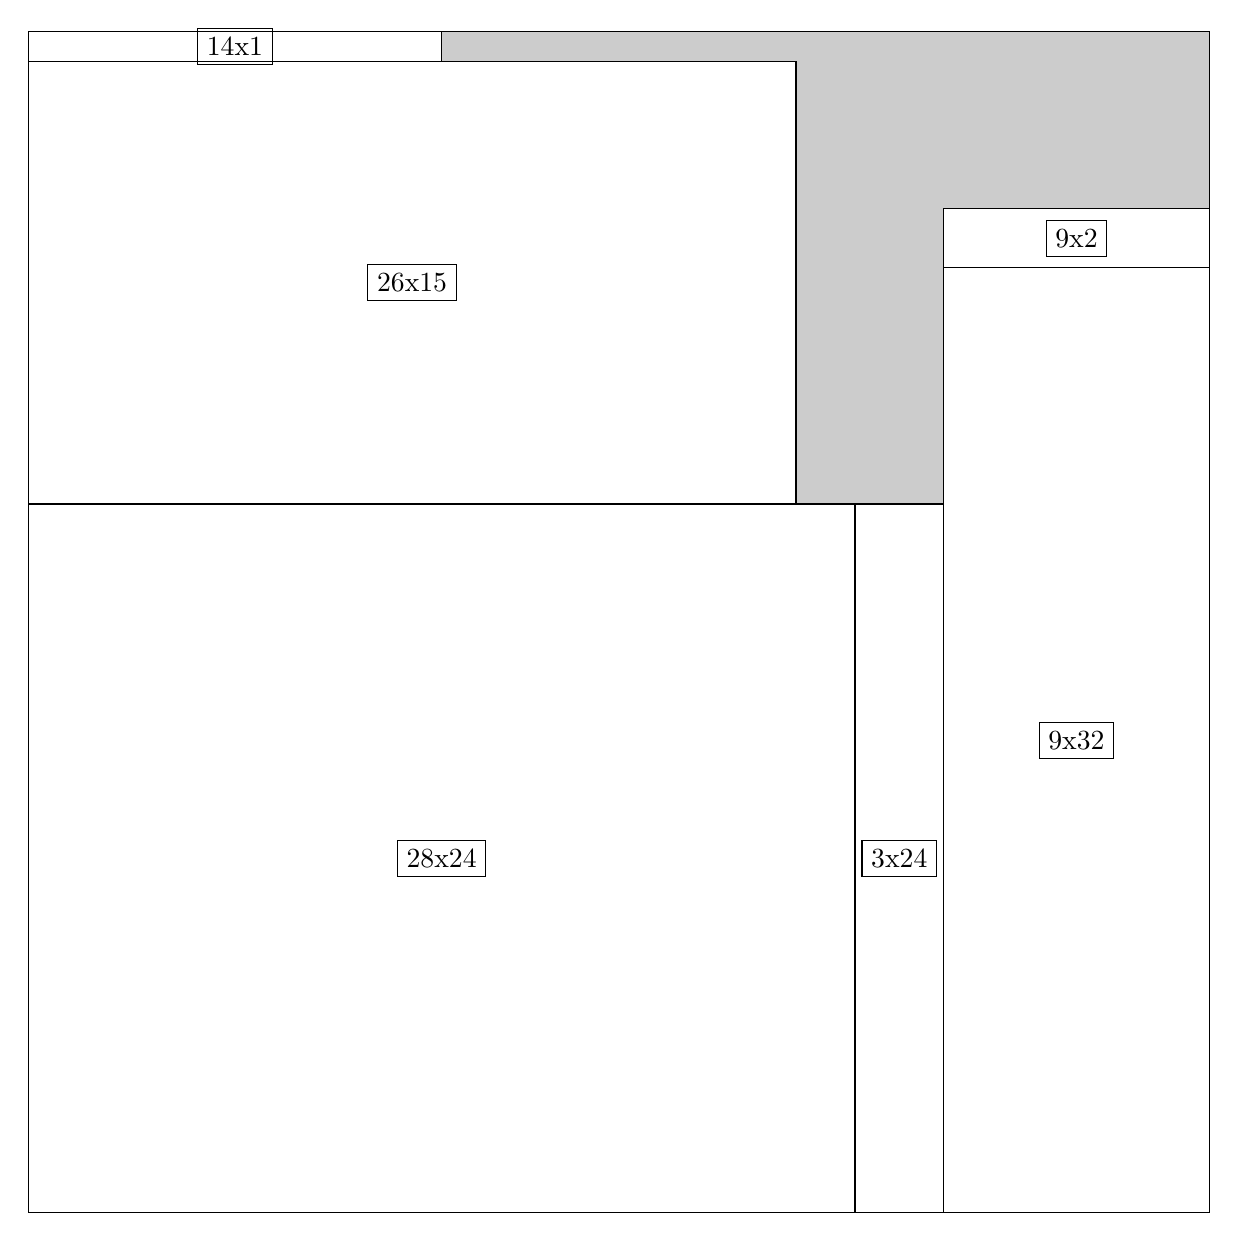
\begin{tikzpicture}[shorten >=1pt,scale=1.0,every node/.style={scale=1.0},->]
\tikzstyle{vertex}=[circle,fill=black!25,minimum size=14pt,inner sep=0pt]
\filldraw[fill=gray!40!white, draw=black] (0,0) rectangle (15.0,15.0);
\foreach \name/\x/\y/\w/\h in {28x24/0.0/0.0/10.5/9.0,9x32/11.625/0.0/3.375/12.0,26x15/0.0/9.0/9.75/5.625,3x24/10.5/0.0/1.125/9.0,9x2/11.625/12.0/3.375/0.75,14x1/0.0/14.625/5.25/0.375}
\filldraw[fill=white!40!white, draw=black] (\x,\y) rectangle node[draw] (\name) {\name} ++(\w,\h);
\end{tikzpicture}


w =28 , h =24 , x =0 , y =0 , v =672
\par
w =9 , h =32 , x =31 , y =0 , v =288
\par
w =26 , h =15 , x =0 , y =24 , v =390
\par
w =3 , h =24 , x =28 , y =0 , v =72
\par
w =9 , h =2 , x =31 , y =32 , v =18
\par
w =14 , h =1 , x =0 , y =39 , v =14
\par
\newpage


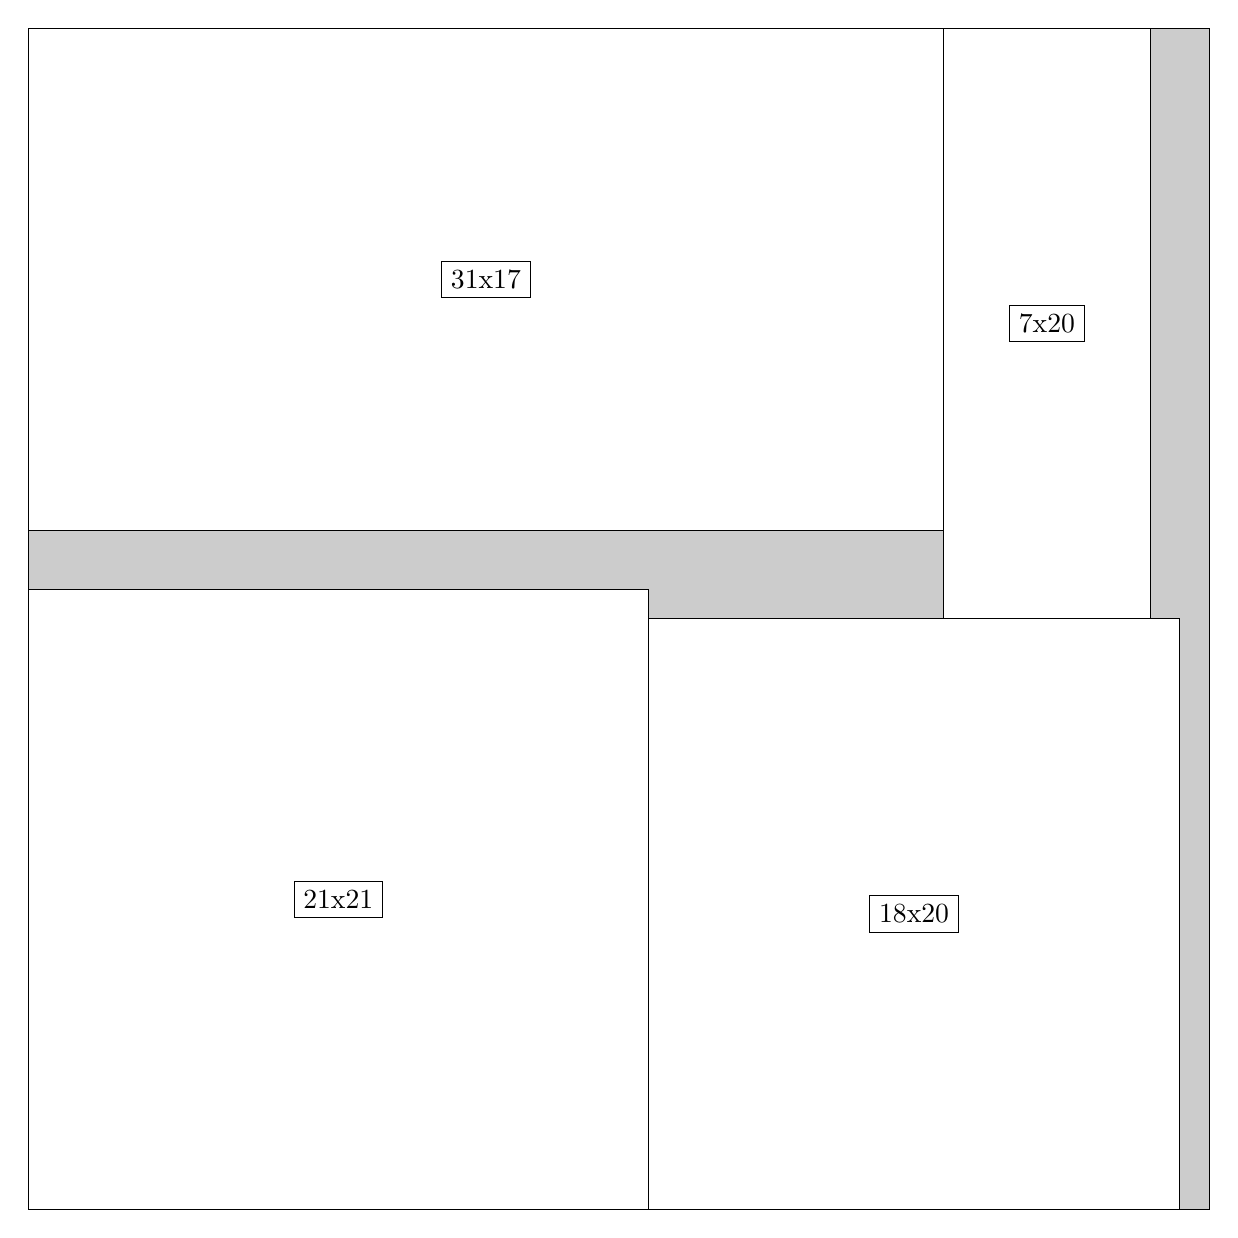
\begin{tikzpicture}[shorten >=1pt,scale=1.0,every node/.style={scale=1.0},->]
\tikzstyle{vertex}=[circle,fill=black!25,minimum size=14pt,inner sep=0pt]
\filldraw[fill=gray!40!white, draw=black] (0,0) rectangle (15.0,15.0);
\foreach \name/\x/\y/\w/\h in {31x17/0.0/8.625/11.625/6.375,21x21/0.0/0.0/7.875/7.875,18x20/7.875/0.0/6.75/7.5,7x20/11.625/7.5/2.625/7.5}
\filldraw[fill=white!40!white, draw=black] (\x,\y) rectangle node[draw] (\name) {\name} ++(\w,\h);
\end{tikzpicture}


w =31 , h =17 , x =0 , y =23 , v =527
\par
w =21 , h =21 , x =0 , y =0 , v =441
\par
w =18 , h =20 , x =21 , y =0 , v =360
\par
w =7 , h =20 , x =31 , y =20 , v =140
\par
\newpage


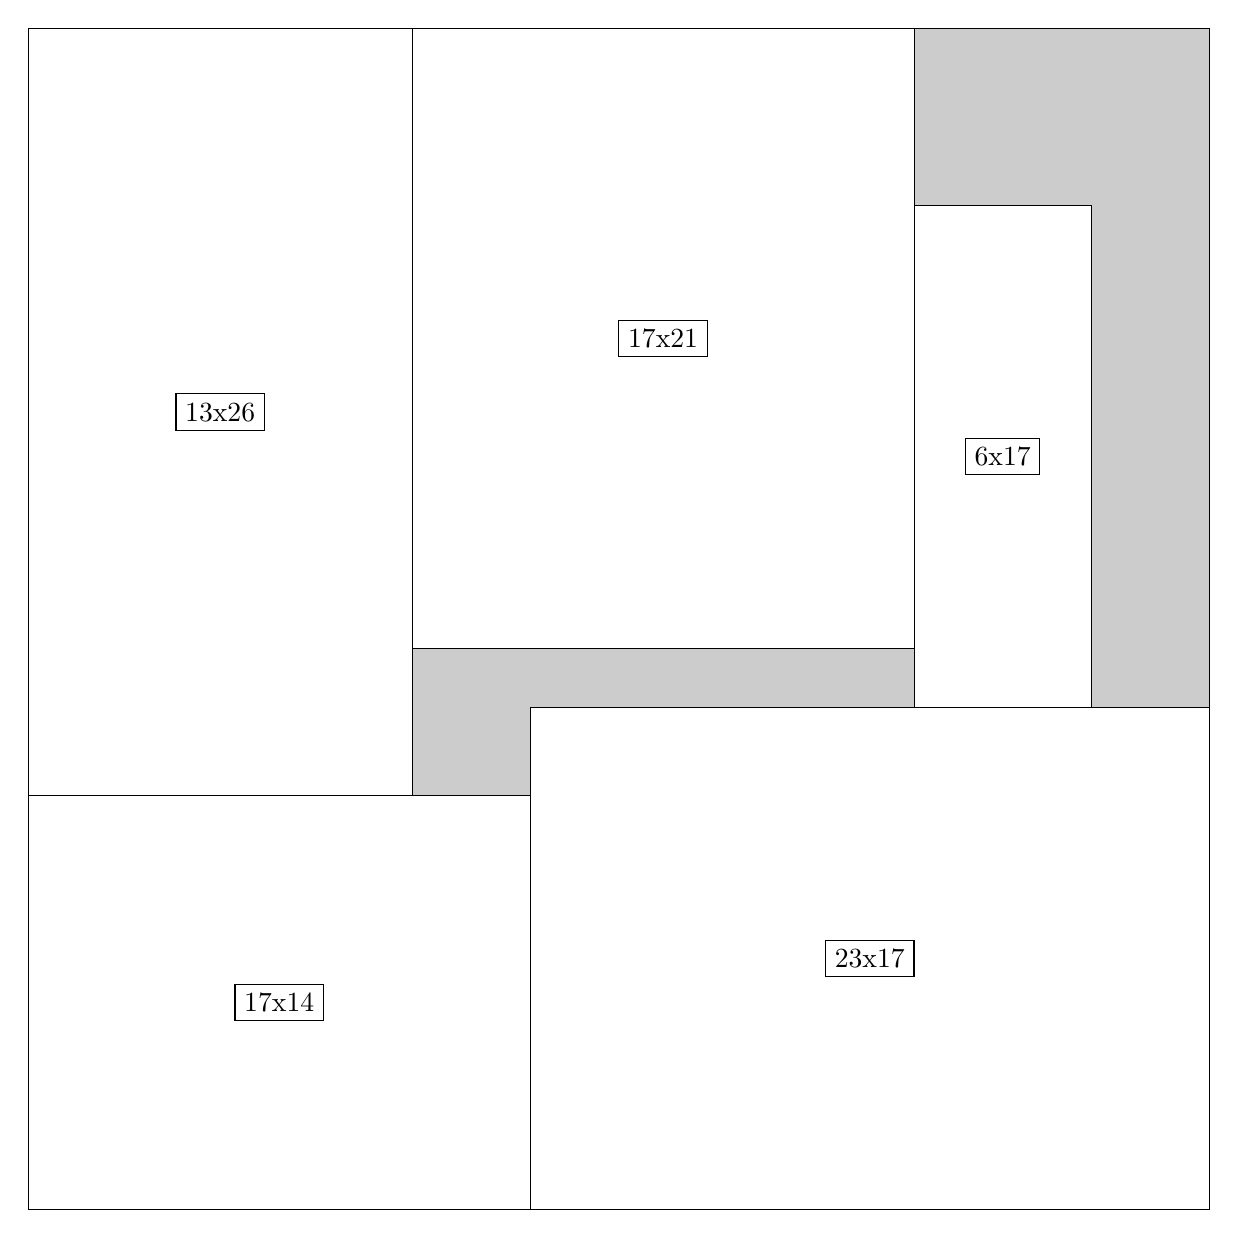
\begin{tikzpicture}[shorten >=1pt,scale=1.0,every node/.style={scale=1.0},->]
\tikzstyle{vertex}=[circle,fill=black!25,minimum size=14pt,inner sep=0pt]
\filldraw[fill=gray!40!white, draw=black] (0,0) rectangle (15.0,15.0);
\foreach \name/\x/\y/\w/\h in {17x14/0.0/0.0/6.375/5.25,23x17/6.375/0.0/8.625/6.375,17x21/4.875/7.125/6.375/7.875,13x26/0.0/5.25/4.875/9.75,6x17/11.25/6.375/2.25/6.375}
\filldraw[fill=white!40!white, draw=black] (\x,\y) rectangle node[draw] (\name) {\name} ++(\w,\h);
\end{tikzpicture}


w =17 , h =14 , x =0 , y =0 , v =238
\par
w =23 , h =17 , x =17 , y =0 , v =391
\par
w =17 , h =21 , x =13 , y =19 , v =357
\par
w =13 , h =26 , x =0 , y =14 , v =338
\par
w =6 , h =17 , x =30 , y =17 , v =102
\par
\newpage


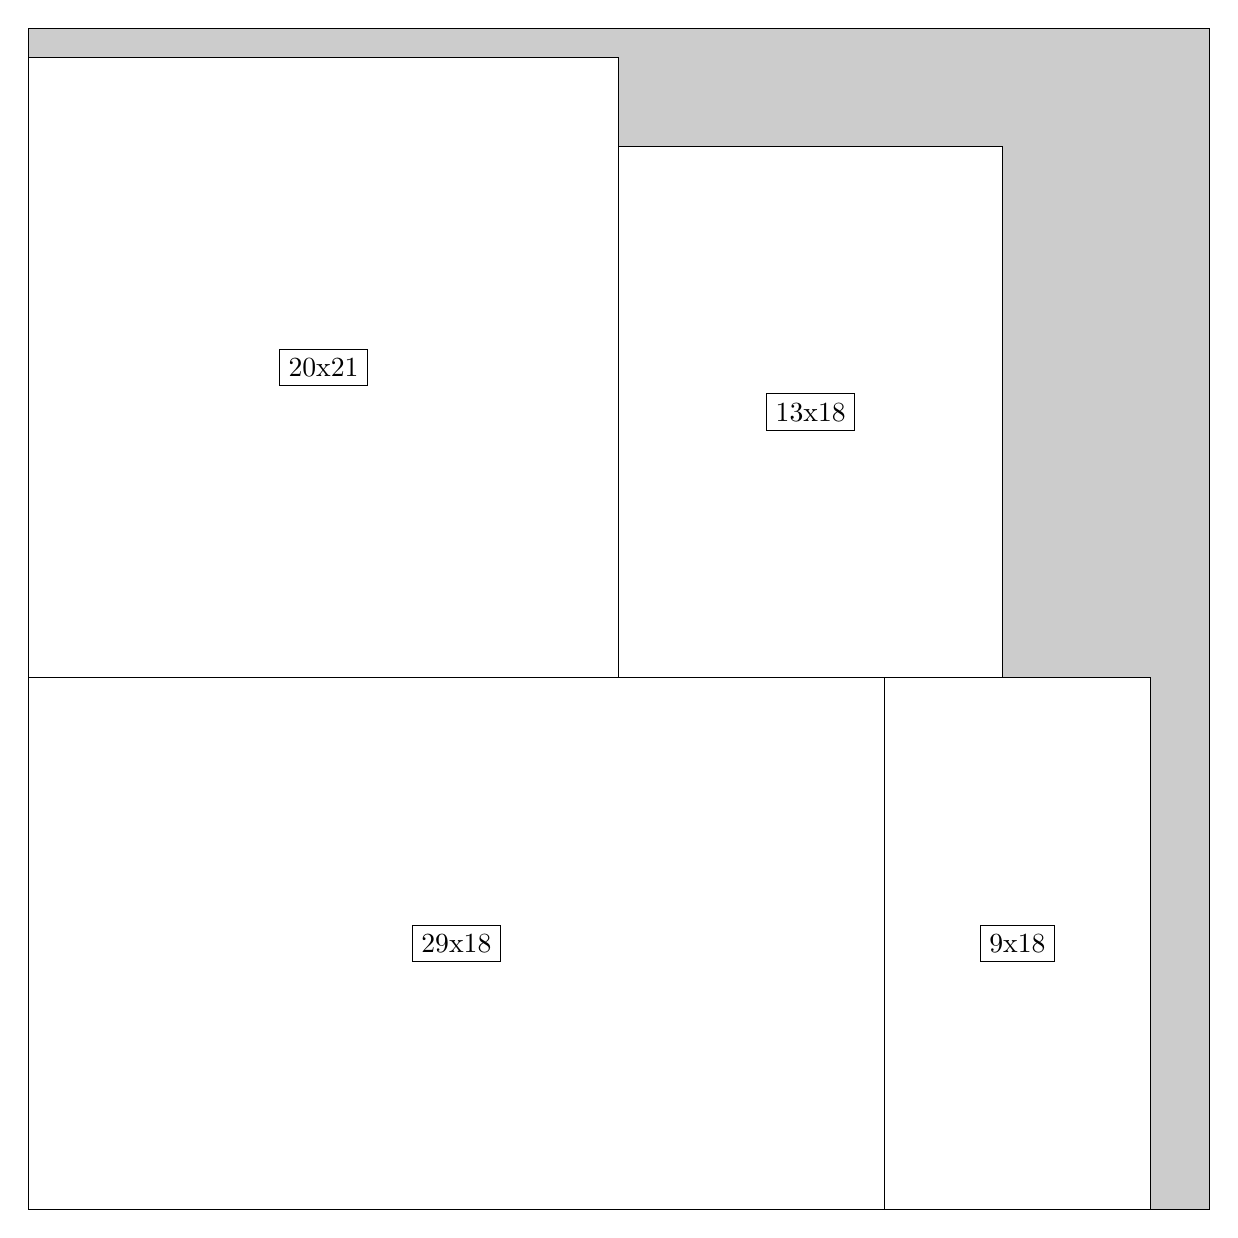
\begin{tikzpicture}[shorten >=1pt,scale=1.0,every node/.style={scale=1.0},->]
\tikzstyle{vertex}=[circle,fill=black!25,minimum size=14pt,inner sep=0pt]
\filldraw[fill=gray!40!white, draw=black] (0,0) rectangle (15.0,15.0);
\foreach \name/\x/\y/\w/\h in {29x18/0.0/0.0/10.875/6.75,20x21/0.0/6.75/7.5/7.875,13x18/7.5/6.75/4.875/6.75,9x18/10.875/0.0/3.375/6.75}
\filldraw[fill=white!40!white, draw=black] (\x,\y) rectangle node[draw] (\name) {\name} ++(\w,\h);
\end{tikzpicture}


w =29 , h =18 , x =0 , y =0 , v =522
\par
w =20 , h =21 , x =0 , y =18 , v =420
\par
w =13 , h =18 , x =20 , y =18 , v =234
\par
w =9 , h =18 , x =29 , y =0 , v =162
\par
\newpage


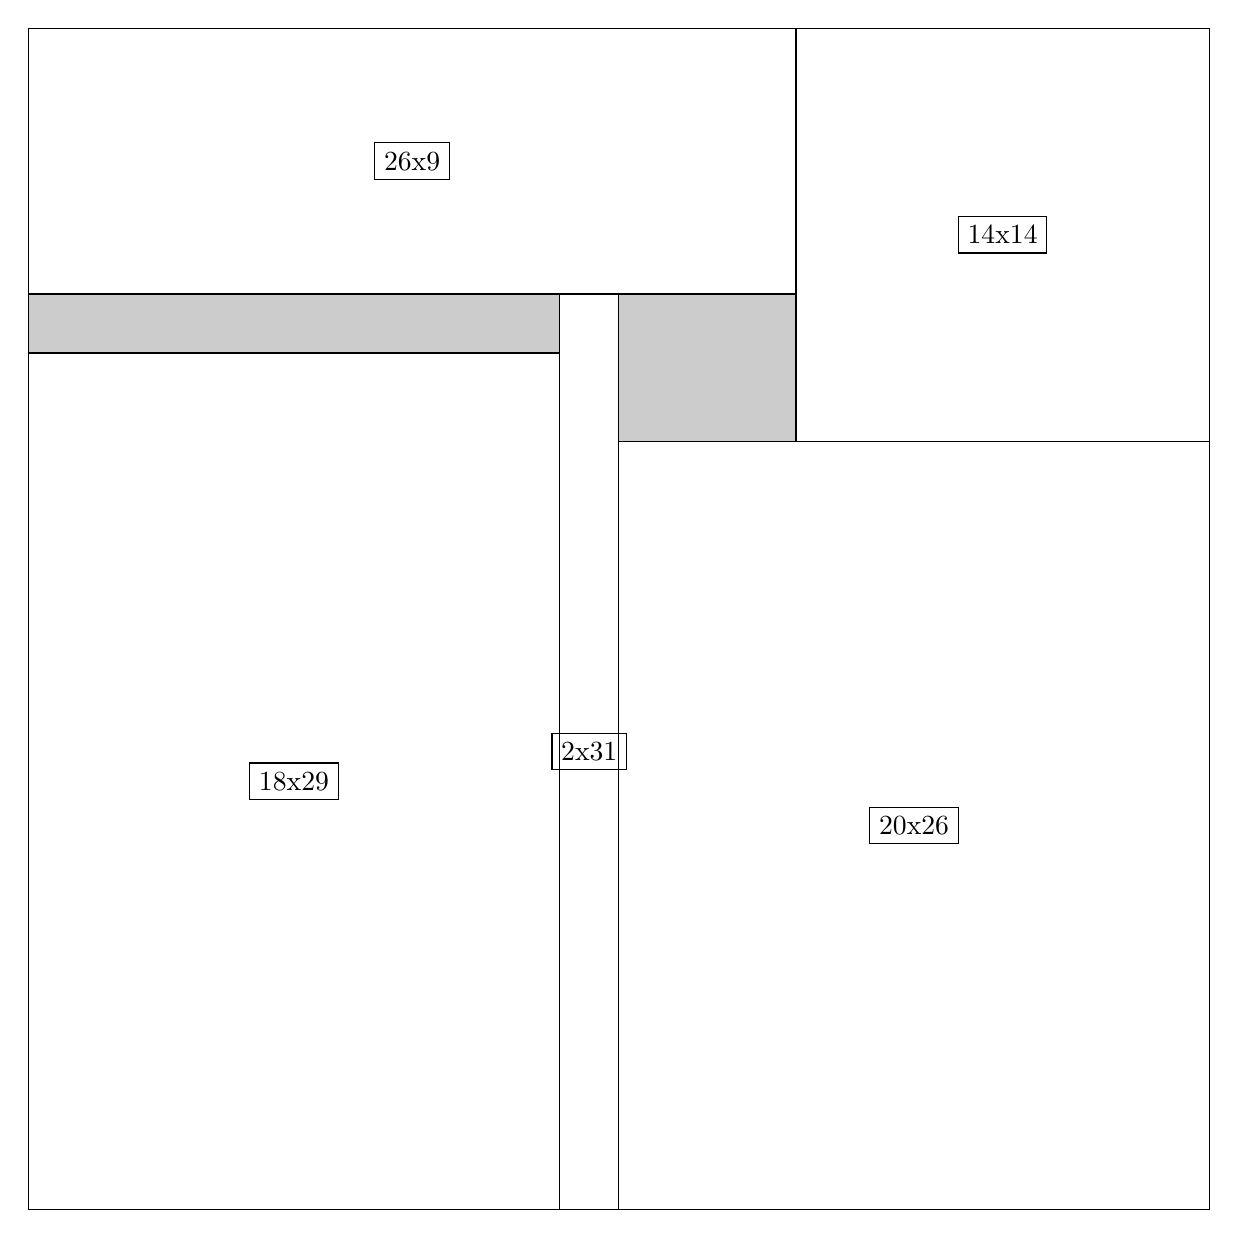
\begin{tikzpicture}[shorten >=1pt,scale=1.0,every node/.style={scale=1.0},->]
\tikzstyle{vertex}=[circle,fill=black!25,minimum size=14pt,inner sep=0pt]
\filldraw[fill=gray!40!white, draw=black] (0,0) rectangle (15.0,15.0);
\foreach \name/\x/\y/\w/\h in {18x29/0.0/0.0/6.75/10.875,20x26/7.5/0.0/7.5/9.75,26x9/0.0/11.625/9.75/3.375,14x14/9.75/9.75/5.25/5.25,2x31/6.75/0.0/0.75/11.625}
\filldraw[fill=white!40!white, draw=black] (\x,\y) rectangle node[draw] (\name) {\name} ++(\w,\h);
\end{tikzpicture}


w =18 , h =29 , x =0 , y =0 , v =522
\par
w =20 , h =26 , x =20 , y =0 , v =520
\par
w =26 , h =9 , x =0 , y =31 , v =234
\par
w =14 , h =14 , x =26 , y =26 , v =196
\par
w =2 , h =31 , x =18 , y =0 , v =62
\par
\newpage


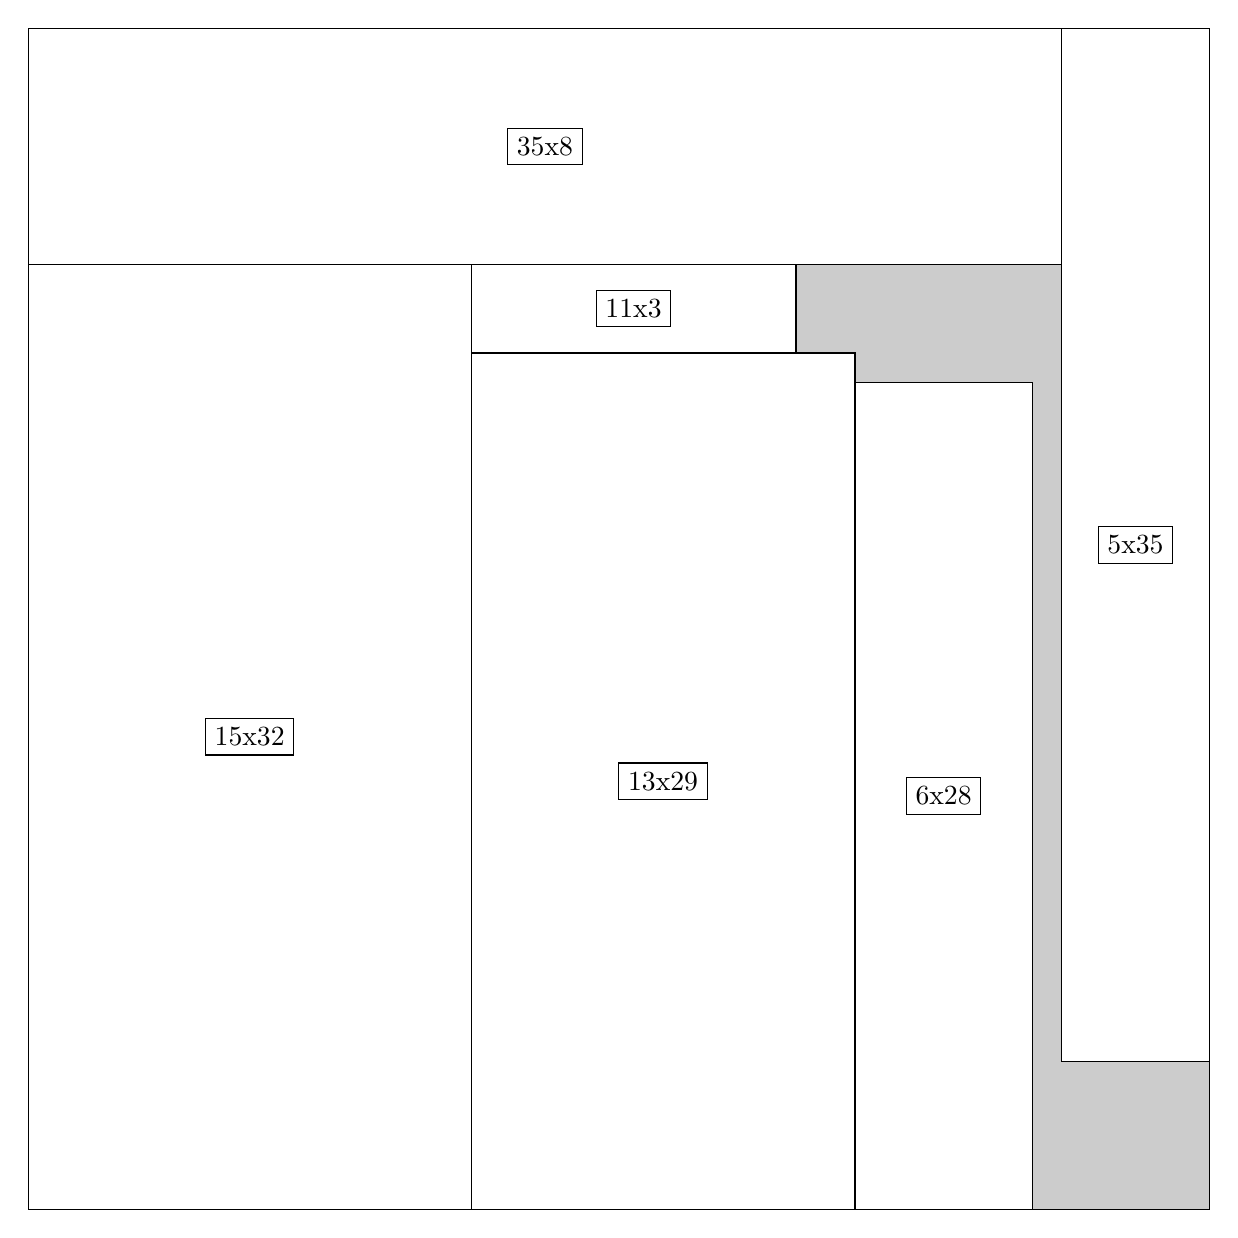
\begin{tikzpicture}[shorten >=1pt,scale=1.0,every node/.style={scale=1.0},->]
\tikzstyle{vertex}=[circle,fill=black!25,minimum size=14pt,inner sep=0pt]
\filldraw[fill=gray!40!white, draw=black] (0,0) rectangle (15.0,15.0);
\foreach \name/\x/\y/\w/\h in {15x32/0.0/0.0/5.625/12.0,13x29/5.625/0.0/4.875/10.875,35x8/0.0/12.0/13.125/3.0,5x35/13.125/1.875/1.875/13.125,6x28/10.5/0.0/2.25/10.5,11x3/5.625/10.875/4.125/1.125}
\filldraw[fill=white!40!white, draw=black] (\x,\y) rectangle node[draw] (\name) {\name} ++(\w,\h);
\end{tikzpicture}


w =15 , h =32 , x =0 , y =0 , v =480
\par
w =13 , h =29 , x =15 , y =0 , v =377
\par
w =35 , h =8 , x =0 , y =32 , v =280
\par
w =5 , h =35 , x =35 , y =5 , v =175
\par
w =6 , h =28 , x =28 , y =0 , v =168
\par
w =11 , h =3 , x =15 , y =29 , v =33
\par
\newpage


\end{document}